% -------------------------------------------------------------------------------------------------
%
%  Skeleton for semester and master thesis reports at the Laboratory for Software Technology.
%  Based on the skeleton provided by the Institute of Robotics and Intelligent Systems.
%
% -------------------------------------------------------------------------------------------------
%
% USAGE:      compile with PDFLaTeX
%
% HISTORY:    - written by Sascha A. Stoeter <stoeter@iris.ethz.ch>, www.stoeter.com, 02.06.2004
%             - modified by Martin Probst, 18.08.2004
%             - extended and adapted for use at LST by Oliver Trachsel, 2007-08-21
% -------------------------------------------------------------------------------------------------
\documentclass[11pt,a4paper]{book}
\usepackage{lstreport}

% -------------------------------------------------------------------------------------------------
% Add needed packages. Some generally useful packages are listed for
% your convenience.
% -------------------------------------------------------------------------------------------------
\usepackage{subfigure}                          % enable the use of subfigures
\usepackage[thickspace,thinqspace]{SIunits}     %
\usepackage[plainpages=false,pdfpagelabels]{hyperref}    % enable hyperlinks in pdf/ps Docs
\usepackage{listings}                           % to embed source code


% UTF8
\usepackage[utf8x]{inputenc} 

% -------------------------------------------------------------------------------------------------
% Select type of thesis
% -------------------------------------------------------------------------------------------------
\renewcommand{\thesistype}{Bachelor}
%\renewcommand{\thesistype}{Diploma}
%\renewcommand{\thesistype}{Master}

% -------------------------------------------------------------------------------------------------
% Set names
% -------------------------------------------------------------------------------------------------
\renewcommand{\thesisauthor}{Marcel Mohler}
\renewcommand{\thesisadvisor}{Zoltán Majó \\ Tobias Hartmann}

%OWN STUFF###############################################################
\usepackage[english]{babel}
\usepackage{color}
\usepackage{textcomp}

% colors
%\definecolor{orange}{rgb}{1,0.5,0}

% Disable single lines at the start of a paragraph (Schusterjungen)

%\clubpenalty = 10000

% Disable single lines at the end of a paragraph (Hurenkinder)

%\widowpenalty = 10000
%\displaywidowpenalty = 10000
 
% allows for colored, easy-to-find todos

\newcommand{\todo}[1]{\textsf{\textbf{\textcolor{orange}{[[TODO: #1]]}}}}

\definecolor{listinggray}{gray}{0.9}
\definecolor{lbcolor}{rgb}{1,1,1}
\lstset{
	backgroundcolor=\color{lbcolor},
	tabsize=4,
	rulecolor=,
	language=java,
  basicstyle=\scriptsize,
  upquote=true,
  aboveskip={1.5\baselineskip},
  columns=fixed,
  showstringspaces=false,
  extendedchars=true,
  breaklines=true,
  prebreak = \raisebox{0ex}[0ex][0ex]{\ensuremath{\hookleftarrow}},
  frame=tb,
  showtabs=false,
  showspaces=false,
  showstringspaces=false,
  identifierstyle=\ttfamily,
  keywordstyle=\color[rgb]{0,0,1},
  commentstyle=\color[rgb]{0.133,0.545,0.133},
  stringstyle=\color[rgb]{0.627,0.126,0.941},
  numbers=left,
  numberstyle=\tiny,
  stepnumber=1,
  numbersep=5pt,
}


%##########################################################################


% -------------------------------------------------------------------------------------------------
% Beginning of the main document body
% -------------------------------------------------------------------------------------------------
\begin{document}

% include all bibtex even if not cited
\nocite{*}

% -------------------------------------------------------------------------------------------------
% Front matter with title page, table of contents, and abstracts 
% -------------------------------------------------------------------------------------------------
\frontmatter

% Title page: set title and date 
\thesistitlepage{Profile Caching for the\\Java Virtual Machine
}{August 2015}

% Abstract must not be longer than one page per language. English and
% German abstracts are mandatory.
\chapter*{Introduction}
\label{c:Introduction}
Virtual Machines like the Java Virtual Machine (JVM) are used as the execution environment of choice for many modern programming languages. 
The VMs interpret a suitable intermediate language (e.g., Java Byte Code for the JVM) and provide the runtime system for application programs and usually include a garbage collector, a thread scheduler and interfaces to the host operating system. 
As interpretation of intermediate code is time-consuming, VMs usually include a \textit{Just-in-time} (JIT) compiler that translates frequently-executed functions or methods to \textit{native} machine code.
\\\\
The JIT compiler executes in parallel to a program's interpretation by the VM and, as a result, compilation speed is a critical issue in the design of a JIT compiler.
Unfortunately, it is difficult to design a compiler such that the compiler produces good (or excellent) code while limiting the resource demands of this compiler. The compiler requires storage, CPU cycles and even on a multi-core processor, compilation may slow down the execution of the application program.
\\\\
Consequently, most VMs adopt a multi-tier compilation system.
%The first tier usually is the interpretation of a method. If this method is executed frequently, the Tier-1 compiler translates this method into native code.
%The Tier-1 compiler implements only a small set of the know optimization techniques and as result, it had good compilation speed but the generated code is far from the output of an optimizing compiler. Such a compiler is usually the Tier-2 compiler, which takes a longer amount of time and produces optimized native code. To determine which methods should be compiled by the Tier-1 (or Tier-2) compiler, the VM profiles the execution of all application programs to identify “hot” methods.
At program startup, all methods are interpreted by the virtual machine (execution at Tier 0). The interpreter gathers execution statistics called profiling and if a method is determined to be executed frequently, this method is then compiled by the Tier 1 compiler. Methods compiled to Tier 1 are then profiled further and based on these profiling information, some methods are eventually compiled at higher tiers.
One of the drawbacks of this setup is that for all programs, all methods start in Tier 0, with interpretation and profiling by the VM. However, for many programs the set of the most used methods does not change from one execution to another and there is no reason to gather profiling information again. 
\\\\
The main idea of this thesis is to cache these profiles from a prior execution to be used in further runs of the same program. 
Having these \textit{cached profiles} available would avoid the JIT compiler to gather the same profiling information again as well as allow it to use more sophisticated profiles early in program execution and prevent recompilations when more information about the method is available. While this in general should influence the peak performance of the program, the hope is to decrease the time the JVM needs to achieve it.
\\\\
This thesis presents an implementation for the latest version of the Java Hotspot Virtual Machine as well as a profound performance analysis using state-of-the-art benchmarks.


%\chapter*{Zusammenfassung}
%Kurzfassung der Arbeit.

% Table of contents
\tableofcontents

% -------------------------------------------------------------------------------------------------
% Main document body
% -------------------------------------------------------------------------------------------------
\mainmatter
\chapter{Overview Hotspot}
\label{c:overview}
This chapter will provide the reader with an overview of the relevant parts of Java HotSpot. The chapter explains the core concepts that are needed to understand the motivation of this thesis and the implementation of the system described in this thesis.

\section{Tiered compilation}
\label{sec:tiered}
As mentioned in the introduction, virtual machines (VMs) like Java HotSpot feature a multi-tier system when compiling methods during execution. 
Java VM's typically use Java Bytecode as input, a platform independent intermediate code generated by a Java Compiler like \texttt{javac} \cite{javac}.
The bytecode is meant to be interpreted by the virtual machine or further compiled into platform dependent machine code (e.g., x86 instructions).
HotSpot includes one interpreter and two different just-in-time compilers with different profiling levels resulting in a total of 5 different \textit{compilation tiers}. Since in literature and the JVM source code use the \textit{tiers} are also called \textit{compilation levels} they will be used synonymously. 
\begin{figure}[ht]
  \begin{center}
    \centering
    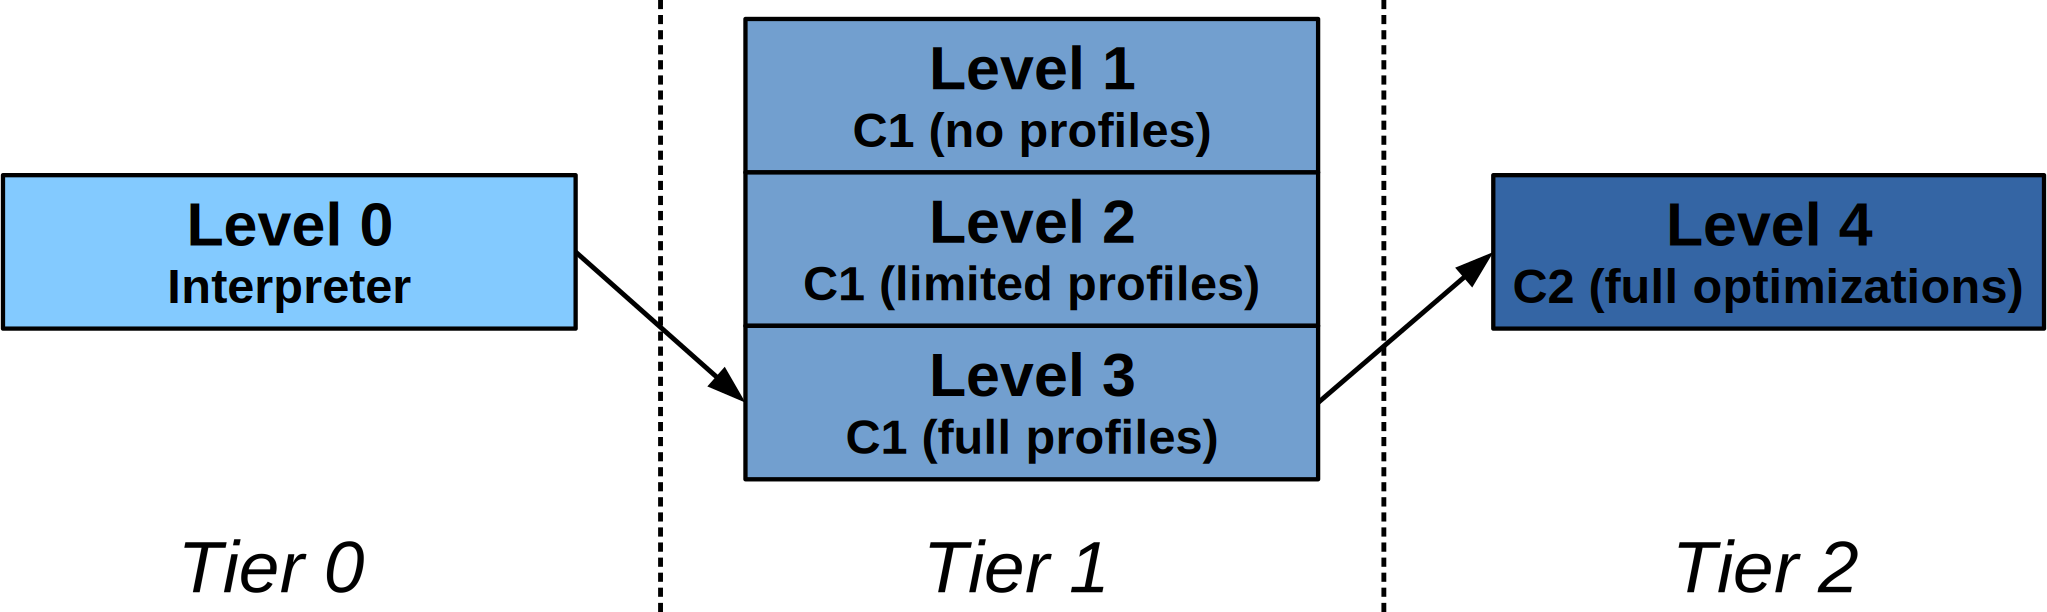
\includegraphics{figures/hs_tiers.png}
    \caption{Overview of compilation tiers}
    \label{f:hs_tiers}
  \end{center}
\end{figure}
\\
All methods start being executed at Tier 0, which denotes the interpreter.
The interpreter performs a template-based replacement, that is, for each bytecode instruction the interpreter emits a predefined assembly code snippet.
During execution, the assembly code is also profiled. The snippets also contain structures to gather method information like execution counters or loop back-branches. a counter exceeds a predefined threshold, the method is considered \textit{hot} and a call back to the JVM is initiated that usually results in a compilation at a higher tier.
\\\\
The standard behavior of HotSpot is to proceed with Level 3 (Tier 3). The method gets compiled with C1, also referred to as \textit{client} compiler.
C1's goal is to provide a fast compilation with a low memory footprint.
The client compiler performs simple optimizations such as constant folding, null check elimination, and method inlining based on the information gathered during interpretation. 
Most of the classes and methods are already used in the interpreter and allow C1 to inline them to avoid costly invocations.
More importantly, information about the program flow and state are gathered. These information contain for example which branches get taken or the final types of dynamically typed objects. 
For example, if certain branches were not taken during execution further compilations might abstain from compiling these branches and replace them with static code to provide a faster method execution time (see the example in Listing \ref{l:branchexample}). The uncommon branch will include an \textit{uncommon trap} which notify the JVM that an assumption does not hold anymore. This then leads to so called \textit{deoptimizations} which are further explained in the separate Section \ref{s:deoptimizations}.
\begin{lstlisting}[float,caption=Example that show potential compilation based on profiling information,label=l:branchexample,language=Java]
public static void m(int i) {
    if ( i == 0 ) { // very common branch (a)
        Math.sin(0);
    } else { // very uncommon branch (b)
        Math.sin(pi + i)
    }
}
// ---------------------------------------------
// If the JVM realizes based on profiling information,
// that branch (a) is taken all the time:
// compiler could compile the method as follows:
// ---------------------------------------------
public static void m(int i) {
    if ( i != 0 ) // very common branch (a)
        // UNCOMMON TRAP, call to JVM
    return 0; // result of sin(0)
}
\end{lstlisting}
\\\\
Level 1 and Level 2 include the same optimizations but offer no or less profiling information and are used in special cases. Code compiled at these levels is significantly faster than Level 3 because it needs to execute none or little instructions creating and managing the profiles. Since the profiles generated by C1 are further used in C2, HotSpot is usually interested in creating full profiles and therefore uses Level 3.
There are, however, rare instances where a compilation of Level 1 or Level 2 is triggered. For example, if enough profiles are available and a method can not be compiled by a higher tier, HotSpot might recompile the method with Tier 2 to get faster code until the higher tier compiler is available again. A compiler can become unavailable if its compilation queue exceeds a certain threshold.
\\\\
More information about C1 can be found in \cite{client_compiler_talk} and \cite{client_compiler}.
\\\\
Eventually, when further compile thresholds are exceeded, the JVM further compiles the method with C2, also known as the \textit{server} compiler.
The server compiler uses the profiles gathered in Tier 0 and Tier 3 and produces highly optimized code. C2 includes far more and more complex optimizations like loop unrolling, common subexpression elimination and elimination of range and null checks. It performs optimistic method inlining, for example by converting some virtual calls to static calls. It relies heavily on the profiling information and richer profiles allow the compiler to use more and better optimizations.
While the code quality of C2 is a lot better than C1 this comes at the cost of compile time. Since a C2 compilation includes 
A more detailed look at the server compiler can be found in \cite{server_compiler}.
Figure \ref{f:hs_tiers} gives a short overview as well as showing the standard transition.
\\\\
The naming scheme \textit{client/server} is due to historical reasons when tiered compilation was not available and users had to choose the JIT compiler via a HotSpot command line flag. The \textit{client} compiler was meant to be used for interactive client programs with graphical user interfaces where response time is more important than peak performance. For long running server applications, the highly optimized but slower \textit{server} compiler was the choice suggested. 
\\\\
Tiered compilation was introduced to improve start-up performance of the JVM.
Starting with the interpreter results in instantaneous execution (i.e. a method is executed right away as there is no delay caused by the method's compilation). Also, there are always methods that are executed infrequently. In these the compilation overhead can exceed the performance gain. C1 allows the JVM to have optimized code available early which then can be used to create a richer profile to be used when compiling with C2. Ideally this profile already contains most of the program flow and the assumptions made by C2 hold. If that is not the case the JVM might need to go back, gather more profiles and compile the method again. In this case, being able to do quick compilations with C1 decreases the amount of C2 recompilations which are even more costly.

\section{Deoptimizations}
\label{s:deoptimizations}
Ideally a method is compiled with as much profiling information as possible.
For example, since the profiling information are usually gathered in Levels 0 and 3, it can happen that a method compiled by C2 wants to execute a branch it never used before (again see Figure \ref{l:branchexample}).
In this case the information about this branch are not available in the profile and therefore have not been compiled into the C2-compiled code.
This is done to allow further even more optimistic optimization and to keep the compiled code smaller. So instead, the compiler places an uncommon trap at unused branches or unloaded classes which will get triggered in case they actually get used at a later time in execution.
\\\\
The JVM then stops execution of that method and returns the control back to the interpreter. This process is called \textit{deoptimization} and considered very expensive. The previous interpreter state has to be restored and the method will be executed using the slow interpreter. Eventually the method might be recompiled with the newly gained information.

\section{On-Stack Replacement}
\label{s:onstackreplacement}
Since the JVM does not only count method invocations but also loop back branches (see also Section \ref{s:compilethresholds}) it can happen that a method is compiled while it is still running and the compiled method is ready before the method has finished.
Instead of waiting for the next method invocation, HotSpot can replace the method directly on the program stack. The JVM sets up a new stack frame for the compiled method which replaces the interpreters stack frame and execution will continue using the native method.
\\\\
This process is called \textit{on-stack replacement} and usually shortened to OSR. The Figure \ref{f:osr} presented in a talk by T. Rodriguez and K. Russel \cite{client_compiler_talk} gives a graphical representation.
The benefits of OSR will become more obvious when looking at the first example in Chapter \ref{c:motivation}.
\begin{figure}[ht]
  \begin{center}
    \centering
    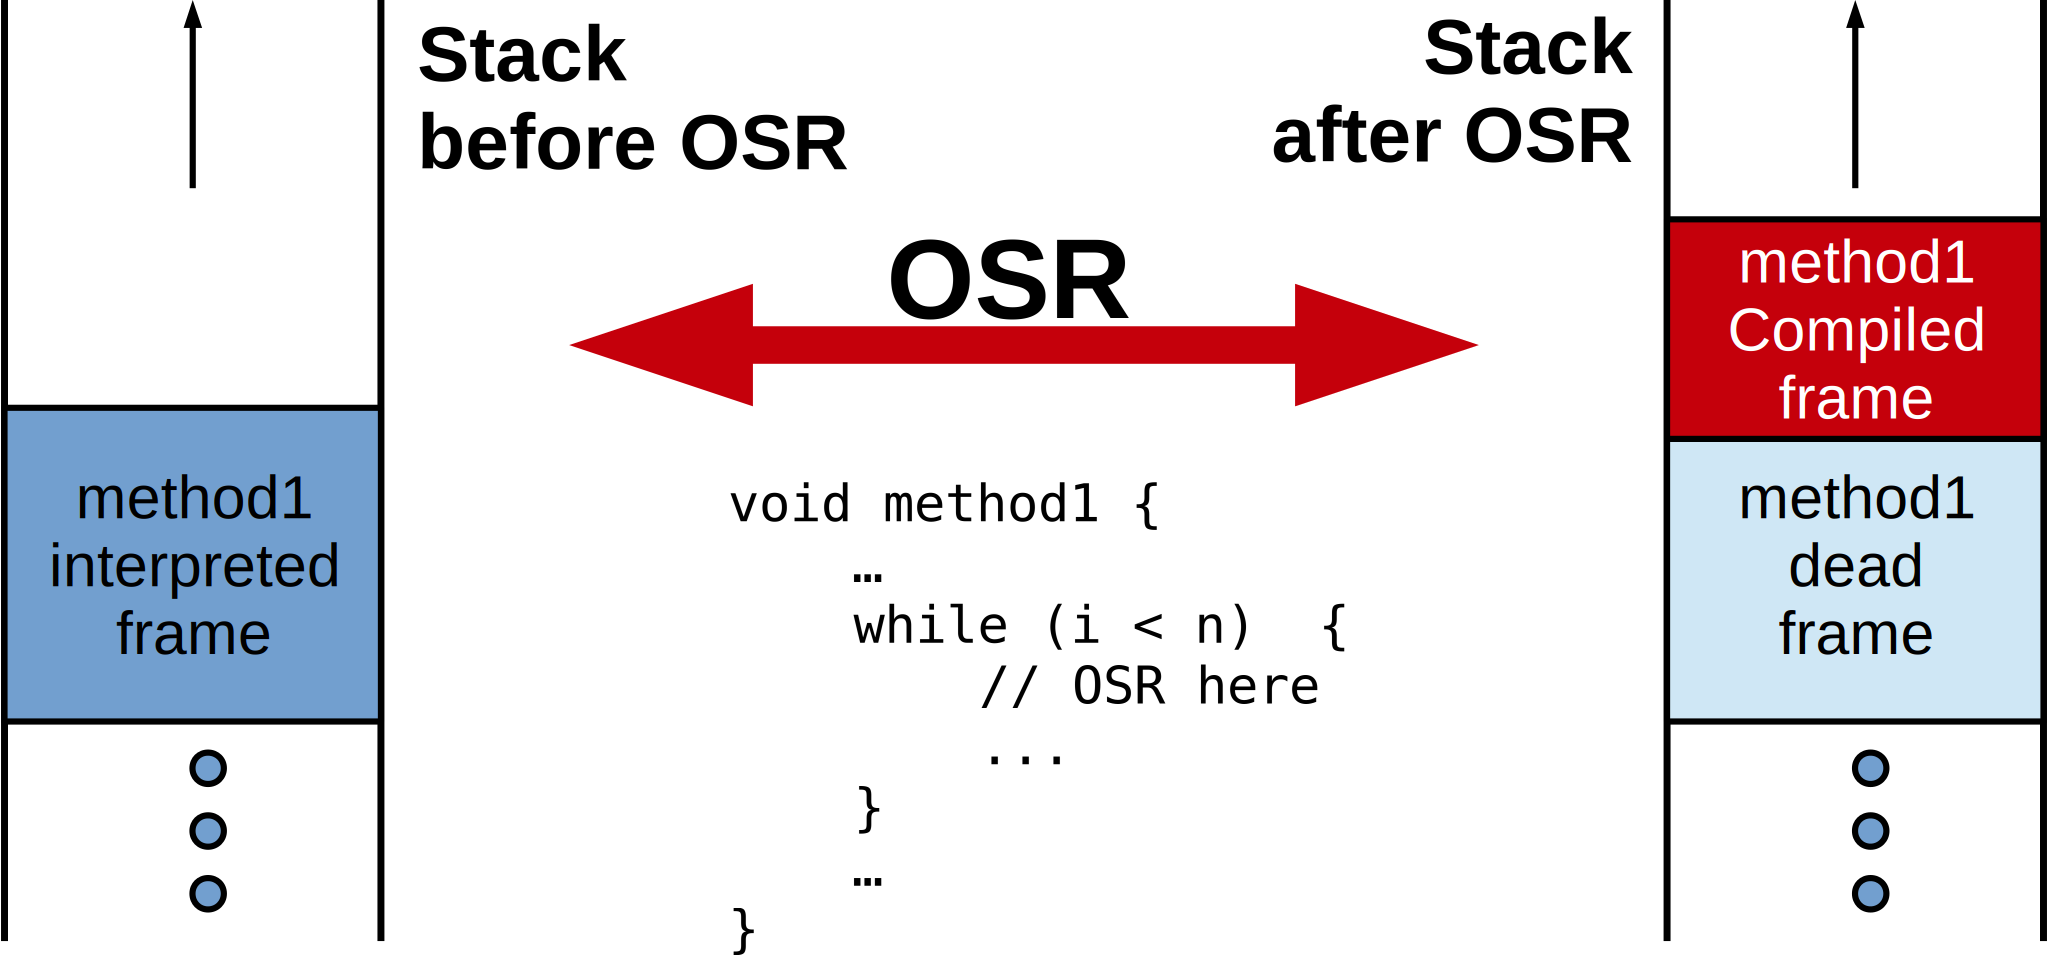
\includegraphics[width=0.6\textwidth]{figures/osr.png}
    \caption{Graphical schema of OSR}
    \label{f:osr}
  \end{center}
\end{figure}
\section{Compile thresholds}
\label{s:compilethresholds}
The transitions between the compilation levels (see Fig. \ref{f:hs_tiers}) are chosen based on predefined constants called \textit{compile thresholds}. When running an instance of the JVM one can specify them manually or use the ones provided. A list of thresholds and their default values relevant to this thesis are given in Appendix \ref{a:compilethresholds}.
The standard transitions from Level 0 to Level 3 and Level 3 to Level 4 happen when the following predicate returns true:
\begin{align*}
& i > TierXInvocationThreshold \ * \ s \\
 || \ (&i > TierXMinInvocationThreshold \ * \ s \ \&\& \ i \ + \ b \ > \ TierXCompileThreshold \ * \ s) 
\end{align*}
where $X$ is the next compile level (3 or 4), $i$ the number of method invocations, $b$ the number of backedges and $s$ a scaling coefficient (default = 1).
The thresholds are relative and individual for interpreter and compiler.
\\\\
On-stack replacement uses a simpler predicate:
$$b > TierXBackEdgeThreshold * s$$
\\\\
Please note that there are further conditions influencing the compilation like the load on the compiler which will not be discussed.


\chapter{Motivation}
\label{c:motivation}
\section{Tiered Compilation in Hotspot}

\section{On Stack Replacement}

\section{Deoptimizations}

\section{Compile Thresholds}

\section{Examples}


\chapter{Implementation / Design}
\label{c:implementation}
This chapter describes the implementation of the cached profiles functionality for HotSpot, written as part of this thesis.
HotSpot is a vital part of the open source Java Platform implementation, \texttt{OpenJDK}, and the source code is available at \url{http://openjdk.java.net/}.
\\\\
Most of the code additions are included in two new classes \texttt{/share/vm/ci/ciCacheProfiles.cpp} and \texttt{/share/vm/ci/ciCacheProfilesBroker.cpp} as well as significant changes to \\\texttt{/share/vm/ci/ciEnv.cpp} and \texttt{/share/vm/compiler/compileBroker.cpp}.
\\
The core functionality is located in \texttt{/share/vm/ci/ciCacheProfiles.cpp}, a class that takes care of setting up the cached profile data-structure as well as providing public methods to check if a method is cached or not. The class \texttt{/share/vm/ci/ciCacheProfilesBroker.cpp} is used before a cached method is compiled. It is responsible for setting up the compilation environment, so the JIT compiler can use the cached profiles.
\\\\
A full list of modified files and the changes can be seen in the webrev at \url{http://mohlerm.ch/b/webrev.01/} or Appendix \ref{a:codechanges}.
The changes are provided in form of a patch for HotSpot version 1aef080fd28d. In the following, the original version is referred to as \textit{baseline}.
\\\\
We will describe and explain the functionality and the implementation design decision in the following sections, ordered by their execution order.

\section{Creating cached profiles}
\label{s:creatingprofiles}
The baseline version of HotSpot already offers a functionality to replay a compilation based on previously saved profiling information.
This is mainly used in case the JVM crashes during a JIT compilation to replay the compilation process and allow the JVM developer to further investigate the cause of this incident.
Apart from this automatic process, there exists the possibility to invoke the profile saving manually by specifying the \texttt{DumpReplay} compile command option per method.
\\\\
We introduce a new method option called \texttt{DumpProfile} as well as a new compiler flag \newline\texttt{-XX:+DumpProfiles} that appends profiling information to a file as soon as a method gets compiled. The first option can be specified as part of the \texttt{-XX:CompileCommand} or \texttt{-XX:CompileCommandFile} flag and allows the user to select single methods to dump their profile. The second command dumps profiles of all compiled methods.
The profile are converted to a string and saved in a simple text file called \textit{cached\_profiles.dat}.
\\\\
The system will only consider compilations of Level 3 or Level 4. Level 1 and Level 2 are rarely used in practice and do only include none or little profiling information. The user can also restrict the profiles to Level 4 ones by using the compiler flag: \texttt{-XX:DumpProfilesMinTier=4}.
\\\\
The dumped profiling information consists of multiple \texttt{ciMethod} entries, \texttt{ciMethodData} entries, and one \texttt{compile} entry. They are separated by line breaks and keywords to make sure the data can be parsed easily. A shortened example of a cached profile can be found in Appendix \ref{a:cacheprofileexample}. The \texttt{ciMethod} entries contain information about the methods used in the compilation and Table \ref{t:cimethod} describes it in more detail. The \texttt{ciMethodData} (see Table \ref{t:cimethoddata}) includes all profiling data about the methods itself to be able to redo the compilation.
The compile entry saves the bytecode index in case of OSR, the level of the compilation and lists all inlining decisions (Table \ref{t:compile}).
\\\\
A method can be compiled multiple times and at different tiers, thus results compilation information for the same method can be dumped multiple times. This is intentional and is taken care of when loading the profiles (see Section \ref{s:initializingprofiles}).
\begin{table}[ht!]
  \caption{content of ciMethod entry in cached profile}
  \label{t:cimethod}
  \begin{center}
    \begin{tabular}{|p{5cm}|p{10.5cm}|} 
      \hline
       \textbf{name} & \textbf{description} \\ \hline\hline
       class\_name,& used to identify the method\\
       method\_name, & \\
       signature & \\ \hline
       invocation\_counter & number of invotations\\ \hline
       backedge\_counter & numbe of counted backedges\\ \hline
       interpreter\_invocation\_count & number of invocations during interpreter phase\\ \hline
       interpreter\_throwout\_count & how many times method was exited via exception while interpreting\\ \hline
       instructions\_size\_name & rough size of method before inlining\\ \hline
    \end{tabular}
  \end{center}
\end{table}
\begin{table}[ht!]
  \caption{content of ciMethodData entry in cached profile}
  \label{t:cimethoddata}
  \begin{center}
    \begin{tabular}{|p{5cm}|p{10.5cm}|} 
      \hline
       \textbf{name} & \textbf{description} \\ \hline\hline
       class\_name,& used to identify the method\\
       method\_name, & \\
       signature & \\ \hline
       state & if data is attached and matured\\ \hline
       current\_mileage & maturity of the oop when snapshot is taken\\ \hline
       orig &  snapshot of the original header\\ \hline
       data & the actual profiling data\\ \hline
       oops & ordinary object pointers, JVM managed pointers to object\\ \hline        
    \end{tabular}
  \end{center}
\end{table}
\begin{table}[ht!]
  \caption{content of compile entry in cached profile}
  \label{t:compile}
  \begin{center}
    \begin{tabular}{|p{5cm}|p{10.5cm}|} 
      \hline
       \textbf{name} & \textbf{description} \\ \hline\hline
       class\_name,& used to identify the method\\
       method\_name, & \\
       signature &\\ \hline
       entry\_bci & byte code index of method\\ \hline
       comp\_level & compilation level of record\\ \hline
       inline & array of inlining information\\ \hline        
    \end{tabular}
  \end{center}
\end{table} 
\section{Initializing cached profiles}
\label{s:initializingprofiles}
The information dumped in step \ref{s:creatingprofiles} can now be used in a next run of that particular program.
To specify that profiles are available, we introduce a new compiler flag \texttt{-XX:+CacheProfiles} that enables the use of previously generated profiles. By default, it reads from a file called \textit{cached\_profiles.dat} but a different file can be specified using \texttt{-XX:CacheProfilesFile=other\_file.dat}.
\\\\
Before any cached profiles can be used the virtual machine has to parse that file and organize the profiles and compile information in a data-structure. This data-structure is completely kept in memory during the whole execution of the JVM to avoid multiple disk accesses.
The parsing process is invoked during boot up of the JVM, directly after the compileBroker gets initialized. This happens before any methods get executed and blocks the main thread of the JVM until finished.
\\\\
As mentioned in Section \ref{s:creatingprofiles}, the file consists of method information, method profiles, and additional compile information. The parser scans the file once and creates a so called \texttt{CompileRecord} for each of the methods that include compilation information in the file. This compile record also includes the list of method information (\texttt{ciMethod}) and their profiling information (\texttt{ciMethodData}).
As mentioned previously, a method's compile information could have been dumped multiple times, which results in multiple \texttt{CompileRecords} for the same method. In this case, HotSpot will only keep the \texttt{CompileRecords} based on the latest data written to the file but never overwrite an existing higher level profile.
Because a profile dumped by the C1 compiler can not be used by the C2 compiler and the other way around, the level of the profile matters as it influences the compile level transitions described in Section \ref{s:cacheprofilesmode}.
And since profiling information only grow, the compilation that happened last contains the richest profile and is considered the best.
This is based on the fact that the richer the profile, the more information about the method execution is known and influences the compiled version of that method. For example, a profile for a method might include data for all its branches and can therefore help avoid running into uncommon traps and trigger deoptimizations.
\\\\
The \texttt{CompileRecord} as well as the lists of methods information and profiles are implemented as an array located in HotSpot's heap space.
They get initialized with a length of 8 and grow when needed. This choice has been done for simplicity and leaves room for further improvements.

\section{Using cached profiles}
\label{s:usingprofiles}
The implementation offers three different modes \texttt{Mode 0}, \texttt{Mode 1}, and \texttt{Mode 2}, that differ in the way they use the cached profiles.
The following paragraph applies to all three modes and I will discuss the differences of the modes in detail in Section \ref{s:cacheprofilesmode}.
\\\\
The idea is to modify the compiler to use cached profiles if available and continue as usual otherwise.
A simplified graphical overview of the program flow for compiling a method with the changes introduced in this thesis can be found in Figure \ref{f:programflow}.
\begin{figure}[ht!]
  \begin{center}
    \centering
    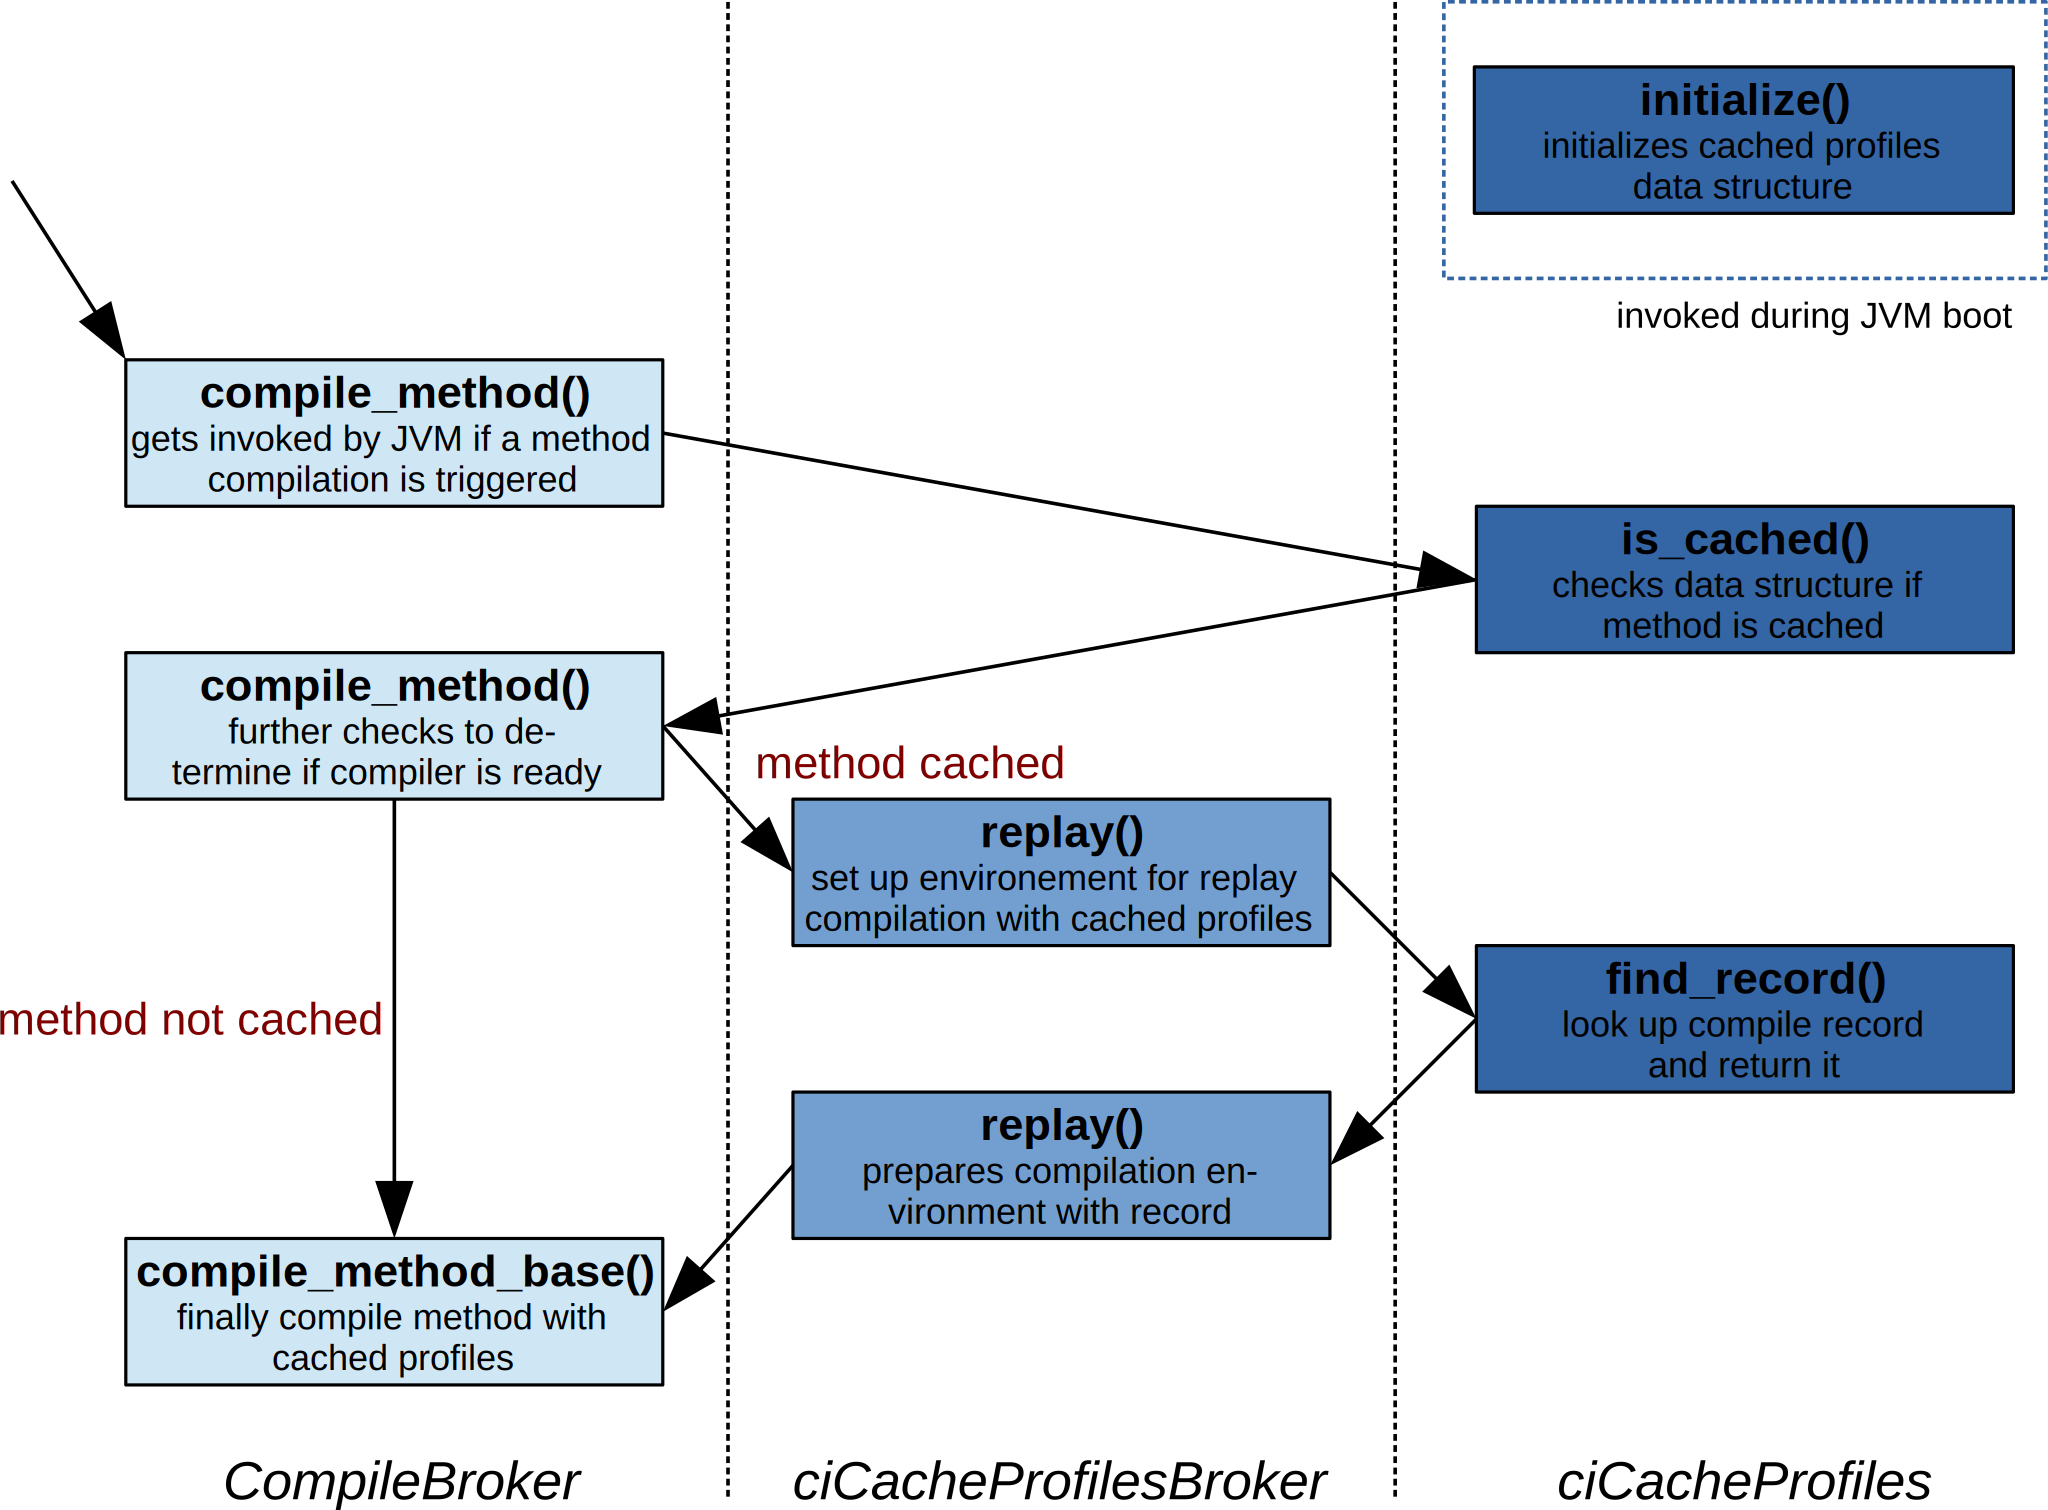
\includegraphics[width=0.8\textwidth]{figures/program_flow.png}
    \caption{program flow for compiling a method}
    \label{f:programflow}
  \end{center}
\end{figure}\\
As mentioned before, once compilation thresholds are exceeded a method is scheduled for compilation. This means that the JVM will invoke a method called \texttt{compile\_method()}, located in the \texttt{compileBroker} class. This method tests if certain conditions hold, for example, it checks if the compile queue is not full or if there is already another compilation of that particular method running.
We extended this method with a call to \texttt{ciCacheProfiles::is\_cached(Method* method)} which does a linear scan through the \texttt{CompileRecord} array data-structure. The method returns either 0 if the method is not cached or returns an integer value, reflecting the compile level, in case a cached profile of this method is available. Because only methods compiled with level 3 or 4 are cached, this call to \texttt{is\_cached()} only gets executed if the compilation request is also of level 3 or higher.\\\\
Depending on the compilation level of the profile, the level of the requested compilation, and the \texttt{CacheProfileMode}, the \texttt{compileBroker} then schedules either a compilation using freshly gathered profiles or calls into \texttt{ciCacheProfilesBroker} to replay the compilation, based on a cached profile. In contrast to cached cached profiles, fresh profiles describe profiles gathered during the current run of the JVM. Since these decisions are different in each mode, I describe them in detail in the next section.
In case the method is not cached, the execution continues like in the baseline version.
Otherwise, the \texttt{ciCacheProfilesBroker} class then initializes the replay environment and retrieves the compile record from \texttt{ciCacheProfiles}. Subsequently, the needed cached profiles get loaded to make sure they are used by the following compilation. \texttt{ciCacheProfilesBroker} then returns the execution to the \texttt{compileBroker}, which continues with the steps needed to compile the method. Again some constraints are checked (e.g. if there is another compilation of the same method finished in the meantime) and a new compile job is added to the compile queue. Eventually the the method is going to be compiled using the cached profiles.
\\\\
Since the implementation is only invoked by the static class \texttt{compileBroker}, \texttt{ciCacheProfiles} and \texttt{ciCacheProfilesBroker} are static classes as well. The \texttt{compileBroker} is solely called by the JVM main thread, therefore there is no need to make the compileRecord data-structure or any of the new implementations thread safe. 

\section{Different usage modes for cached profiles}
\label{s:cacheprofilesmode}
The implementation of cached profiles offers 3 different modes, which distinguish from each other in the transitions between the compilation tiers.
The motivation as well as the advantages and disadvantages of the modes are described in the following three subsections.
While \texttt{Mode 0} and \texttt{Mode 1} are similar except for the compile thresholds, \texttt{mode2} differs significantly.
Figure \ref{f:hs_tiers_thresholds} provides a graphical overview of the differences in the compilation tier transitions of the modes.
\begin{figure}[h]
  \begin{center}
    \centering
    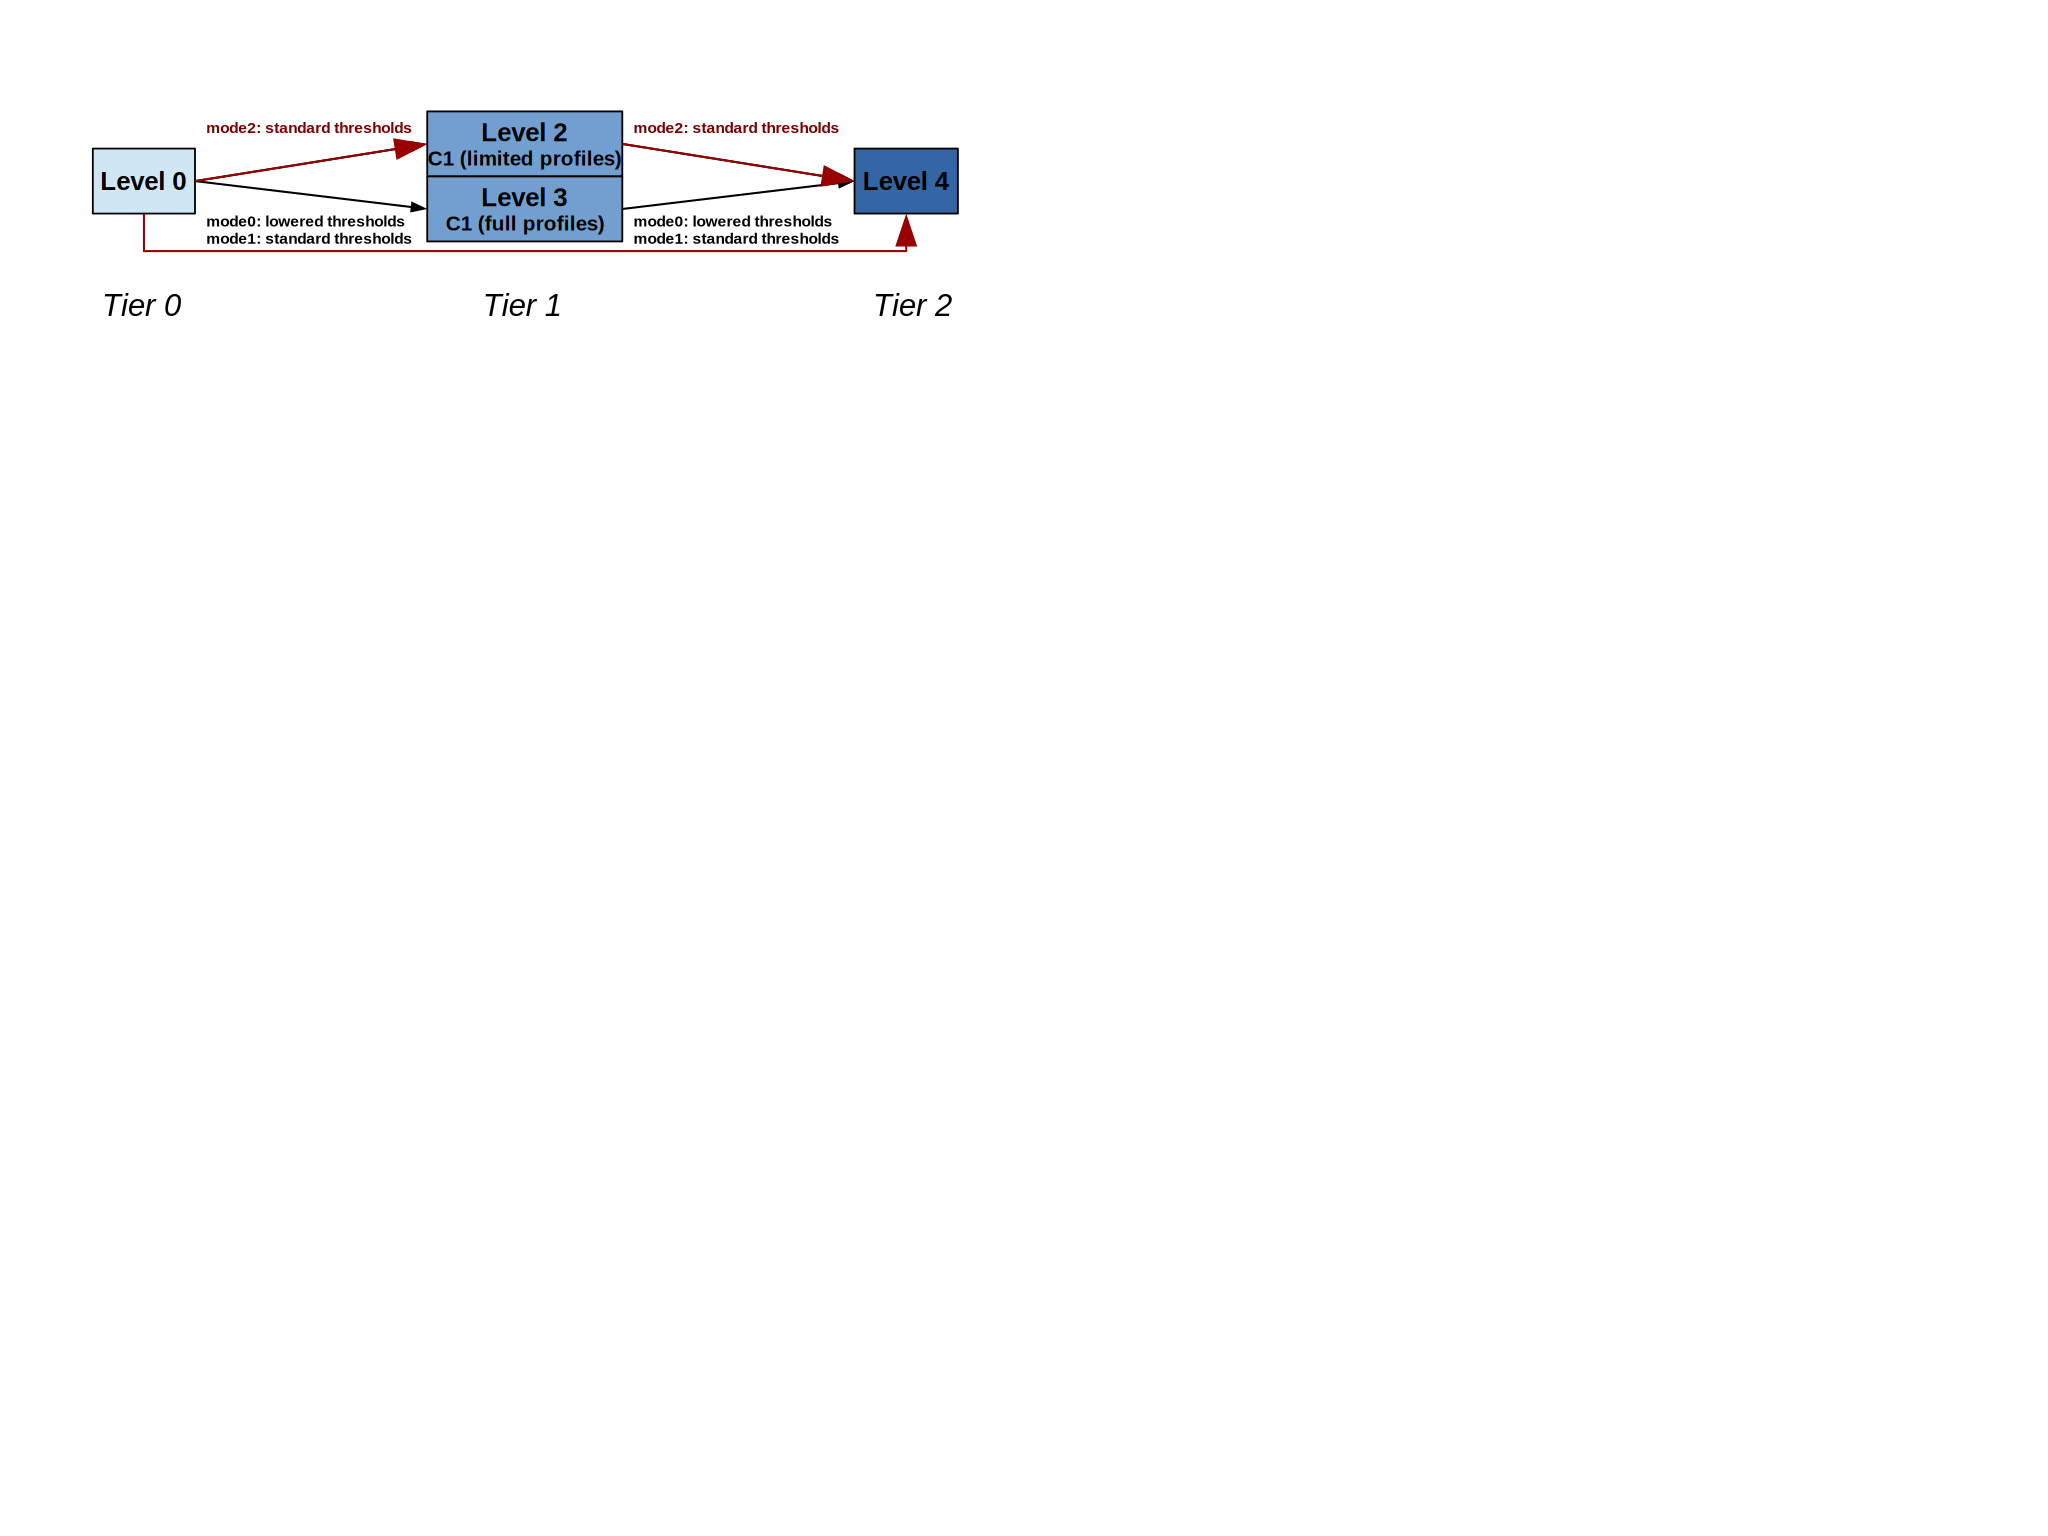
\includegraphics{figures/hs_tiers_threshold.png}
    \caption{Tier transitions of different modes}
    \label{f:hs_tiers_thresholds}
  \end{center}
\end{figure}\\
All three modes have advantages and disadvantages and their performance is evaluated in Chapter \ref{c:performance}. Since depending on the methods, different modes might perform best, it is up to the JVM user to decide which mode he or she wants to use. Because \texttt{Mode 2} is the most conservative one, which does not modify thresholds it is considered the default mode and used if not further specified.

\subsection{Compile Thresholds lowered (Mode 0)}
\label{s:mode0}
The first mode is based on the consideration that a method that has a profile available does not require profiling anymore. Therefore, the compile thresholds (see Section \ref{s:compilethresholds}) of these methods are lowered. If the cached method has a C2 profile, all thresholds are lowered, in case of a C1 profile, only the thresholds that affect the tiers below and equal to Tier 3. This differentiation is done to prevent an increase in early C2 compilations using fresh profiles. Because a lower Tier 4 threshold would mean, that a method which only got compiled at Tier 3 when creation the profile, might now trigger a Tier 4 compilation very early. At this point, the fresh profiles generated by the Tier 3 compiled version are still immature. Using them to compile with Tier 4 results in code that includes only limited profiling information, which causes costly deoptimizations when used. 
\\\\
By default, the thresholds are lowered to 1\% of their original values but the threshold scaling can be modified with the JVM parameter: \texttt{-XX:CacheProfilesMode0ThresholdScaling=x.xx}. 1\% results in the level 3 invocation counter being reduced from 200 to 2. This means that the method will be interpreted once but then directly trigger a compilation on the next invocation.
\\\\
Since the interpreter also handles class loading, this decision has been made to avoid the need of loading classes in C1 or C2 which was considered out of the scope for this thesis. HotSpot expects classes of standard libraries to be loaded in a very specific order. Moving class loading to C1 or C2 would mess with that order and can therefore not be done without huge changes to the JVM.
\\\\
In \texttt{Mode 0}, the JIT compiler will always use a cached profile for compilations of Level 3 or Level 4 in case there is a cached profile which has been generated by a compiler of the same level. However, if a method to be compiled on Level 3 has a cached profile available for Level 4, the compiler will skip the C1 compilation and immediately compile with C2. In this case, HotSpot directly uses the highly optimized version generated by C2 and in an ideal case the method will need less time to reach peak performance.
\\\\
However, since the thresholds of all methods with cached profiles get lowered and some of the C1 compilations are promoted to C2 compilations, the C2 compiler is put under heavy load. Especially during startup of a program, where many compilations happen naturally, C2 might not be able to handle all these requests at the same time and the compile queue fills up. This might negatively affect performance and is analyzed in Section \ref{s:perf_compilequeue}.

\subsection{Unmodified Compile Thresholds (Mode 1)}
\label{s:mode1}
\texttt{Mode 1} is doing exactly the same as \texttt{Mode 0} but does not lower the compilation thresholds of methods with cached profiles.
This is done to decrease the load increase on C2 as mentioned in Subsection \ref{s:mode0}.
Apart from this change \texttt{Mode 1} has the same behaviour as \texttt{Mode 0}.
\subsection{Modified C1 stage (Mode 2)}
\label{s:mode2}
Both modes mentioned before use cached profiles as soon as a compilation of level 3 and 4 are triggered. Since the thresholds for level 3 are smaller than the level 4 thresholds (see Appendix \ref{a:compilethresholds}) a method reaching a level 3 threshold could actually trigger a level 4 compilation, if the cached profile is one of level 4. So even if \texttt{Mode 1} is used and the thresholds are untouched, C2 might get overloaded since compilations occur earlier.
\\\\
\texttt{Mode 2} has been designed to make as little changes as possible to the tiered compilation and prevent C2 being more used than usual. It does so by keeping the original tiered compilation steps and compilation thresholds and compiles methods with C1 prior to C2. But since there are already profiles available, there is no need to run at Tier 3 to generate full profiles but instead it uses Tier 2.
Tier 2 does the same optimizations but offers only limited profiles like method invocation and backbranch counters. They are needed to know when to trigger the C2 compilation and therefore Tier 1 can not be used. 
By avoiding Tier 3 and using Tier 2 instead methods spend less time in code gathering profiling information and therefore method execution is considered about 30\% faster \cite{code_atp_hpp}.
Eventually, if the Tier 4 thresholds are reached, the method is compiled using C2 and the cached profiles. This still maintains the benefit from having more complete profiles available early but avoids modifying thresholds which could result in a very different load to the compiler. 
\\\\
The above only makes sense if the cached profile is a C2 profile.
If only a C1 profile is available, C1 should gather fresh, full profiles since they might be needed in C2 later. HotSpot will then only use the cached profile during the C1 compilation and then use the generated profiles for possible C2 compilations.
In theory this transition is considered rare, because if a method has not been compiled with C2 when creating the profile it is unlikely to get compiled with C2 in the future.

\section{Problems}
\label{s:problems}
If the profiles generated by multiple runs of the program deviate sharply it is likely that a cached profile does not fit to the current execution. In this case the compiled version would still trigger many deoptimizations and the method could end up having even worse performance since it's going to use the profile over and over again.
For each method, the JVM maintains a deoptimization counter. Cache profiles are used if the counter is below a certain limit. If they are above that limit a standard compilation using freshly gathered profiles will be used instead.
The limit is 10 to allow a small number of recompilations. This could for example be useful when the method is deoptimized due to classes not being loaded. The value of 10 seems reasonable for all executed measurements.
\section{Debug output}
\label{s:debugoutput}
For debugging and benchmarking purposes four debug flags are implemented, that can be used along with \texttt{-XX:+CacheProfiles}.
\begin{table}[ht]
  \centering
 % \caption{}
  \label{t:debugflags}
  \begin{center}
    \begin{tabular}{| l | p{9.0cm} |}
       \hline
       \textbf{flag} & \textbf{description} \\ \hline\hline
       -XX:+PrintCacheProfiles & enable command line debug output for cached profiles\\ \hline
       -XX:+PrintDeoptimizationCount & prints amount of deoptimizations when the JVM gets shut down\\ \hline
       -XX:+PrintDeoptimizationCountVerbose & prints total the amount of deoptimizations on each deoptimization\\ \hline
       -XX:+PrintCompileQueueSize & prints the total amount of methods in the compile queue each time a method gets added \\ \hline
    \end{tabular}
  \end{center}
\end{table}

 


\chapter{Performance}
\label{c:performance}
This section evaluates the performance of the cached profile implementation using modern benchmark suites. The goal is to provide indicators on the performance influence and try to analyze where this performance influence comes from. Since we try to decrease warmup time and decrease the number of deoptimizations 
\section{Setup}
\label{s:perf_setup}
To provide reliable and comparable results all tests were done on a single node of the Data Center Observatory provided by ETH \cite{ethdco}.
A node features 2 8-Core AMD Opteron 6212 CPUs running at 2600 MHz with 128 GB of DDR3 RAM and a solid state disk.
The node is running Fedora 19 and GCC 4.8.3. All JDK builds got created on the node itself.
\\\\
To compare performance the following benchmarks were used:
\begin{enumerate}
  \item \textbf{SPECjvm 2008:} A benchmark suite developed by Standard Performance Evaluation Corporation for measuring the performance of the Java Runtime Environment \cite{specjvm}.  I use version 2008 and I run a subset of 17 out of a total of 21 benchmarks. 4 are omitted due to incompatibility with openJDK 1.9.0.
  \\
  Once finished, SPECjvm prints out the number of operations per minute. This is used to compare the performance and higher is better.
  \item \textbf{Octane 2.0:} A benchmark developed by Google to measure the performance of JavaScript code found in large, real-world applications \cite{octane}. Octane runs on Nashorn, a JavaScript Engine on top of Hotspot. The version used is 2.0 and consists of 17 individual benchmarks of which 16 are used.
  \\
  Octane gives each benchmark a score reflecting the performance, the higher the score, the better the performance.
\end{enumerate}
The benchmarking process was automated using a number of self-written python scripts. The graphs in this chapter always show the arithmetic mean of 50 runs and the error bars display the 95\% confidence intervals.

\section{Benchmark performance}
\label{s:perf_benchmark}
The main goal of cached profiles is to improve the startup performance of the JVM. Having a rich profile from an earlier execution will allow the JIT compiler to use a highly optimized version right from the beginning.
We expect the modes to produce different results. The following list suggests reasons for these performance differences:
\begin{itemize}
  \item Some benchmarks might profit from compiling methods very early and therefore favor Mode 0.
  \item That could however result in many early compilations that overload the compilation queue resulting in worse performance. In this case Mode 1 will perform better than Mode 0.
  \item In case a cached profile can not be used (i.e. the limit of 10 deoptimizations was reached) the JVM needs to use freshly generated profiles. In case the thresholds were lowered (Mode 0) this compilation might have happened very early and only very incomplete profiles were available. This effect is less a problem when Mode 1 is used.
  \item Mode 2 keeps the steps of the original tiered compilation and is considered the most conservative mode. It puts the same load on the compile queue than the baseline version.
\end{itemize}
I will start by looking at SPECjvm since it offers ways to focus on the warmup. An individual description of each benchmark being used can be found in Appendix \ref{a:specjvm_benchmark}.
\subsection{SPECjvm warmup performance}
\label{s:perf_specjvm_warmup}
The longer a program is running the less impact a faster warmup has. Considering most benchmarks include a warmup phase which does not count towards the final score simply running the complete benchmark suite is not an option.
Instead I limited SPECjvm to 1 single operation which, depending on the benchmark take around 6 to 40 seconds.
Additionally, the JVM gets restarted between each single benchmark to prevent methods shared between benchmarks being compiled already.
\\\\
I run each benchmark with all cached profiling features disabled. This run is called the \textit{baseline} and displays the current openJDK 1.9.0 performance.    
\\\\ 
I then use a single benchmark run where I dump the profiles to disk. This run is not limited to a single operation and instead uses the default values of the benchmark. By default the benchmark is limited by time and runs for about 6 minutes. The idea is that these profiles include information that are usually not available during warmup and result in less deoptimizations and better code quality.
\\\\
These profiles are then used in 3 individual runs using the introduced \texttt{-XX:CacheProfiles} flag. Each run is using one of the 3 different CacheProfilesModes.
\begin{figure}[ht]
  \begin{center}
    \centering
    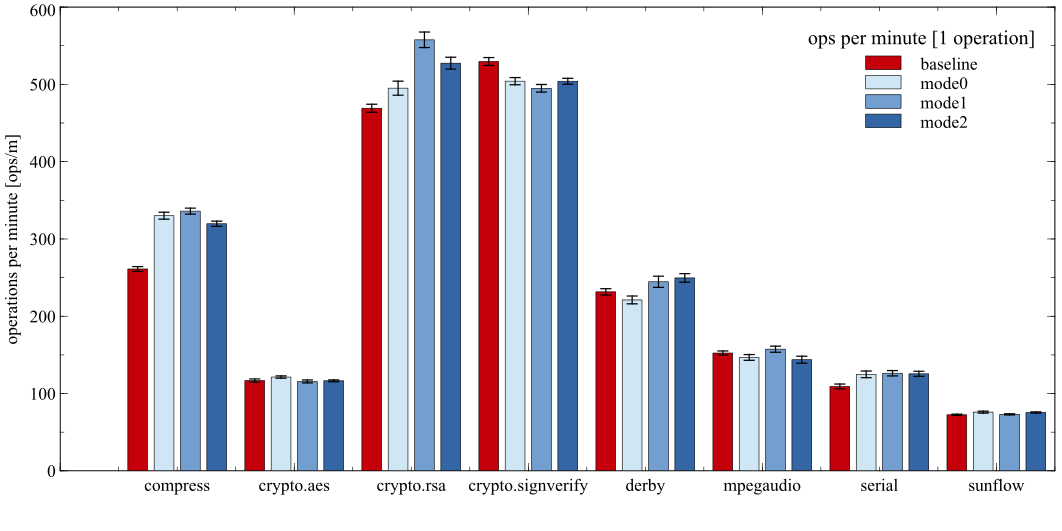
\includegraphics[width=1.0\textwidth]{figures/others_warmup.png}
    \caption{SPECjvm benchmarks on all different modes}
    \label{f:others_warmup}
  \end{center}
\end{figure}
\begin{figure}[ht]
  \begin{center}
    \centering
    \includegraphics[width=1.0\textwidth]{figures/scimark_warmup.png}
    \caption{SPECjvm scimark benchmarks on all different modes}
    \label{f:scimark_warmup}
  \end{center}
\end{figure}

\begin{figure}[ht]
  \begin{center}
    \centering
    \includegraphics[width=1.0\textwidth]{figures/all_warmup_variation.png}
    \caption{Relative performance from baseline for all SPECjvm benchmarks}
    \label{f:all_warmup_variation}
  \end{center}
\end{figure}
Figures \ref{f:others_warmup} and \ref{f:scimark_warmup} shows the number of operations per minute, measured for each benchmark individually. Note, that the operations per minute is not to be confused with the \textit{1 operation }of the benchmark itself.
Figure \ref{f:all_warmup_variation} summarizes the results by showing the relative performance compared to the baseline.
\\\\
The individual benchmarks show different effects on performance. Taking the average of all modes, we see a performance increase up to around 34\% in the compress benchmark (Mode 1) and a performance decrease of down to 20\% in scimark.sparse.large (Mode 0).
\\\\
Interestingly, the performance differences between the modes is not the same when comparing the individual benchmarks. For example in crypto.rsa Mode 0 clearly performs worst but in scimark.sparse.small it performs best.
JVM performance is known to be very hard to predict and it seems not to be different when cached profiles are used. On average the performance of the benchmark warmup is improved by 2.64\%, 3.37\%, and 2.67\% for Mode 0, Mode 1 and Mode 2.
\\\\
Between the three different modes there is no clear \textit{winner}. Each mode wins and looses in certain benchmarks against the others in terms of performance. However, in 12 out of 17 benchmarks at least one of the CacheProfileModes improves performance. 
\\\\
We will take a more detailed look at single benchmarks later in this chapter. 
\subsection{Octane performance}
\label{s:perf_octane}
Since the individual Octane benchmarks are rather short (most of them run for between 4 and 30 seconds) and there is no way to run a fixed number of iterations (without modifying the Octane source) we run the Octane benchmarks completely. We still split up the execution in the individual benchmarks to achieve many JVM restarts. The rest of the setup is identical to the SPECjvm run in Section \ref{s:perf_specjvm_warmup}.
\\\\
The absolute results are shown in Figure \ref{f:octane} and a relative comparison with the baseline in Figure \ref{f:octane_variation}.
Compared to SPECjvm the Octane performance is more scattered. The richards benchmark increases by around 50\% in Mode 0 while navierstockes decreases by around 25\% in Mode 1. In most benchmarks (9 out of 14) Mode 0 performs worst.
We assume this is related to the increased load of the compile queue and will therefore take a more detailed look at this in Section \ref{s:perf_compilequeue}. The performance of the two other modes is better in most benchmarks, but in total only 6 out of 14 benchmarks result in a performance improvement in at least one mode.

\begin{figure}[ht]
  \begin{center}
    \centering
    \includegraphics[width=1.0\textwidth]{figures/octane.png}
    \caption{Octane benchmarks on all different modes}
    \label{f:octane}
  \end{center}
\end{figure}

\begin{figure}[ht]
  \begin{center}
    \centering
    \includegraphics[width=1.0\textwidth]{figures/octane_variation.png}
    \caption{Relative performance from baseline for all Octane benchmarks}
    \label{f:octane_variation}
  \end{center}
\end{figure}
\section{Deoptimizations}
\label{s:perf_deoptimizations}
We are still eager to figure out where the performance increase and decrease come from.
We aim to lower the time needed for warmup by compiling methods earlier and or at lower tiers but also expect to decrease the number of deoptimizations by having more complete profiles early, which ideally results in better compiled code quality. To measure the total amount of deoptimizations we added a new compiler flag \texttt{-XX:+PrintDeoptimizationCount}.
The total number of deoptimizations of the SPECjvm benchmarks is shown in Figure \ref{f:others_warmup_deopt} and Figure \ref{f:scimark_warmup_deopt}. The Octane numbers are drawn in Figure \ref{f:octane_deopt}.
Again, we also included graphs that show the number of deoptimizations relative to the baseline runs in Figure \ref{f:all_warmup_variation_deopt} and Figure \ref{f:octane_variation_deopt}.
\\\\
The measurements show, that when using Mode 1 or Mode 2, we are able to reduce the deoptimizations significantly in all benchmarks except one (gameboy). In Mode 0 there is a clear difference between SPECjvm and Octane. While in SPECjvm the number of deoptimizations is similar to the other modes, in Octane Mode 0 on average increases the number by 30\%. Mode 0 also has the worst performance for Octane and we assume the amount of deoptimizations to be one of the reasons for that regression.
\\\\
And while a low deoptimization number is a good indication of the increased code quality for methods being compiled with cached profiles we could not find a direct correlation between number of deoptimizations and the performance results.
\\\\
One possible reason is that the amount of deoptimizations does not necessarily describe the performance impact. Especially when considering multi-threaded systems there can be a huge number of deoptimizations in performance uncritical threads that are avoided by using cached profiles and therefore heavily reduce the total counter. But if there is one very important method in a performance critical thread, that has executions that are not reflected in the cached profiles, this method could trigger only very few deoptimizations but still influence performance significantly.
\begin{figure}[ht]
  \begin{center}
    \centering
    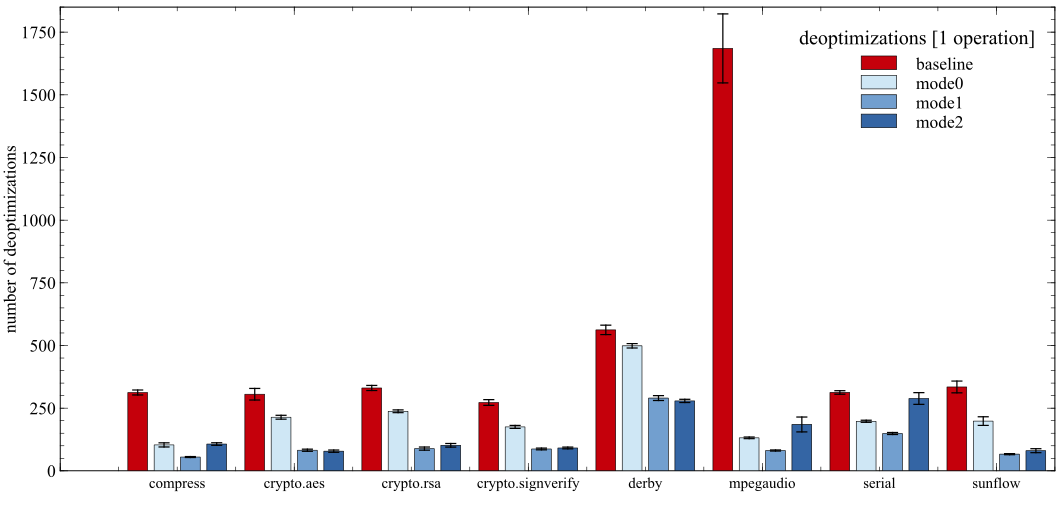
\includegraphics[width=1.0\textwidth]{figures/others_warmup_deopt.png}
    \caption{SPECjvm deoptimizations of all modes}
    \label{f:others_warmup_deopt}
  \end{center}
\end{figure}

\begin{figure}[ht]
  \begin{center}
    \centering
    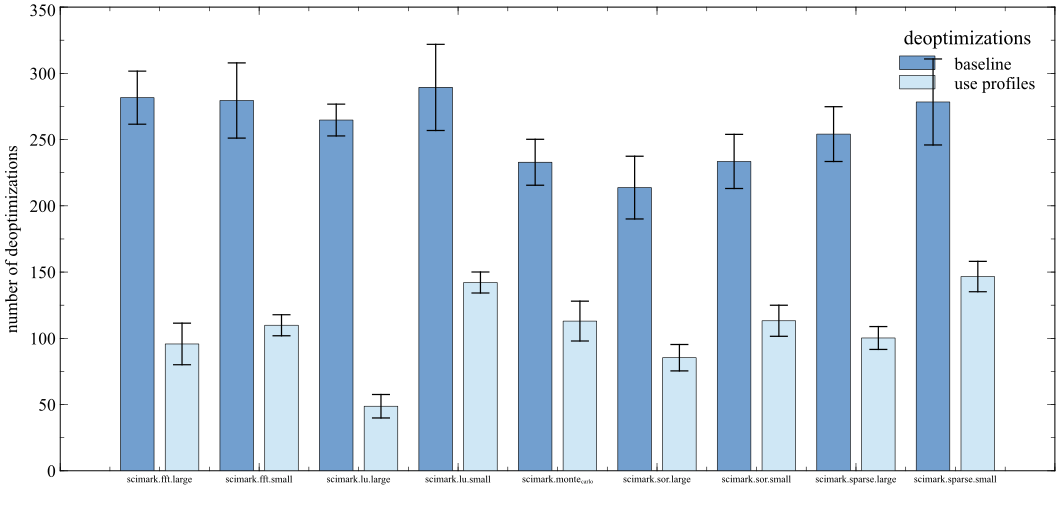
\includegraphics[width=1.0\textwidth]{figures/scimark_warmup_deopt.png}
    \caption{SPECjvm scimark deoptimizations of all modes}
    \label{f:scimark_warmup_deopt}
  \end{center}
\end{figure}

\begin{figure}[ht]
  \begin{center}
    \centering
    \includegraphics[width=1.0\textwidth]{figures/all_warmup_variation_deopt.png}
    \caption{Relative deoptimizations from baseline for all SPECjvm benchmarks}
    \label{f:all_warmup_variation_deopt}
  \end{center}
\end{figure}

\begin{figure}[ht]
  \begin{center}
    \centering
    \includegraphics[width=1.0\textwidth]{figures/octane_deopt.png}
    \caption{Octane deoptimizations of all modes} 
    \label{f:octane_deopt}
  \end{center}
\end{figure}



\begin{figure}[ht]
  \begin{center}
    \centering
    \includegraphics[width=1.0\textwidth]{figures/octane_variation_deopt.png}
    \caption{Relative deoptimizations from baseline for all Octane benchmarks}
    \label{f:octane_variation_deopt}
  \end{center}
\end{figure}

\clearpage
\section{Effect on compile queue}
\label{s:perf_compilequeue}
When designing the different CacheProfilesModes, we thought that lowering the compilation thresholds will increase the load on the compiler, especially early in program execution. This results in the compiler not being able to handle all requests immediately and the compile queue fills up. This could delay execution of compiled methods and therefore decrease performance.
\\\\
We added a new HotSpot flag \texttt{-XX:+PrintCompileQueueSize} which allows us to trace the current number of methods that are scheduled for compilation. We selected 6 indidividual benchmarks and printed their C1 and C2 compile queue for all three CacheProfileModes in Figure \ref{f:octane_queue_richards_separate_c1} to Figure \ref{f:octane_queue_deltablue_separate_c2}.
Keep in mind that the reason for the runs using cached profiles starting their compilations on later time stamps is because they need to parse the cached profile file first.
The selected benchmarks and the reason why an individual analysis was performed are listed below:
\begin{itemize}
  \item \textbf{Octane Richards:} This benchmarks achieved the highest performance benefit from using cached profiles in all three modes. We are interested to see if the compile queue load differs from worse performing benchmarks.
  \item \textbf{Octane EarleyBoyer:} This is a benchmark were \texttt{Mode 1} performs significantly better than the other two modes. Does the compile queue give as any indication why this is the case?
  \item \textbf{Octane NavierStokes:} Navierstokes has a 8\% performance increase in \texttt{Mode 2} but a 25\% performance decrease in \texttt{Mode 0} and \texttt{Mode 1}. Motivation is the same as for EarleyBoyer.
  \item \textbf{Octane Deltablue:} This benchmark achieves the highest performance loss from using cached profiles in all three modes. Together with the best benchmark (Richards) does the load on the compile queue give any indication of performance?
  \item \textbf{SPECjvm compress:} Compress is the best performing SPECjvm benchmark when using cached profiles. 
  \item \textbf{SPECjvm scimark.sparse.large:} This is the worst performing SPECjvm benchmark when using cached profiles. 
\end{itemize}
We realize that analyzing the compile queue does not really help us understanding the performance variations when using cached profiles.
The graphs showing the C1 compile queue size over time do not significantly differ, neither from the baseline, nor is there a difference between the individual modes.
The C2 compile queue graphes show different courses but we can not connect this with the benchmark performance.
\\\\
Figure \ref{f:octane_queue_richards_separate_c2} show the C2 compile queue of the Octane Richards benchmark. As expected, due to removing steps from the tiered compilation, we increased the load on C2 in \texttt{Mode 0} and \texttt{Mode 1} with compile queue peaks at around 20 scheduled compilations. Nevertheless, these modes achieve close a performance of close to 50\% better than the baseline. \texttt{Mode 2} which was designed to keep the original tiered compilation steps unmodified does not have these peaks but nevertheless achieves similar performance.
\\\\
EarleyBoyer's compile queue is displayed in Figure \ref{f:octane_queue_richards_separate_c2}. \texttt{Mode 1} performs better than the other two modes and compared to \texttt{Mode 0} seems to put even more pressure on the compile queue.
It is interesting that in this particular benchmark even the baseline version puts a lot of pressure on the compile queue early on.
\\\\
In Figure \ref{f:octane_queue_navierstokes_separate_c2} we see NavierStokes' compile queue. \texttt{Mode 2} performs best but we could not derive any indications why this is the case from looking at the queue size.
\\\\
The Deltablue benchmark shown in Figure \ref{f:octane_queue_deltablue_separate_c2} has the worst performance when using cached profiles but the compile queue size looks very similar to the one of the Richards benchmark, where performance is significantly better.
\\\\
We will omit looking at the SPECjvm benchmarks since they do not offer any new insights. The graphs can be found in the Appendix \ref{a:additional_graphs}.
\\\\
The detailed analysis of the compile queue shows that our thoughts about the effect on the compile queue were not unfounded for most of the selected benchmarks. However, we were not able to relate these influences to actual performance effects. Especially, overloading the compile queue does not necessarily negatively affect performance.
\\\\
This indicates that the performance differences are even more related to the actual code quality.
% --------------------------- Octane Richards Queue ------------------
\begin{figure}[ht]
  \begin{center}
    \centering
    \includegraphics[width=1.0\textwidth]{figures/octane_queue_richards_separate_c1.png}
    \caption{C1 Compile queue size over time Octane Richards benchmark}
    \label{f:octane_queue_richards_separate_c1}
  \end{center}
\end{figure}
\begin{figure}[ht]
  \begin{center}
    \centering
    \includegraphics[width=1.0\textwidth]{figures/octane_queue_richards_separate_c2.png}
    \caption{C2 Compile queue size over time Octane Richards benchmark}
    \label{f:octane_queue_richards_separate_c2}
  \end{center}
\end{figure}
% --------------------------- Octane EarleyBoyer Queue ------------------
\begin{figure}[ht]
  \begin{center}
    \centering
    \includegraphics[width=1.0\textwidth]{figures/octane_queue_earleyboyer_separate_c1.png}
    \caption{C1 Compile queue size over time Octane EarleyBoyer benchmark}
    \label{f:octane_queue_earleyboyer_separate_c1}
  \end{center}
\end{figure}
\begin{figure}[ht]
  \begin{center}
    \centering
    \includegraphics[width=1.0\textwidth]{figures/octane_queue_earleyboyer_separate_c2.png}
    \caption{C2 Compile queue size over time Octane EarleyBoyer benchmark}
    \label{f:octane_queue_earleyboyer_separate_c2}
  \end{center}
\end{figure}
% --------------------------- Octane NavierStokes Queue ------------------
\begin{figure}[ht]
  \begin{center}
    \centering
    \includegraphics[width=1.0\textwidth]{figures/octane_queue_navierstokes_separate_c1.png}
    \caption{C1 Compile queue size over time Octane NavierStokes benchmark}
    \label{f:octane_queue_navierstokes_separate_c1}
  \end{center}
\end{figure}
\begin{figure}[ht]
  \begin{center}
    \centering
    \includegraphics[width=1.0\textwidth]{figures/octane_queue_navierstokes_separate_c2.png}
    \caption{C2 Compile queue size over time Octane NavierStokes benchmark}
    \label{f:octane_queue_navierstokes_separate_c2}
  \end{center}
\end{figure}
% --------------------------- Octane DeltaBlue Queue ------------------
\begin{figure}[ht]
  \begin{center}
    \centering
    \includegraphics[width=1.0\textwidth]{figures/octane_queue_deltablue_separate_c1.png}
    \caption{C1 Compile queue size over time Octane Deltablue benchmark}
    \label{f:octane_queue_deltablue_separate_c1}
  \end{center}
\end{figure}
\begin{figure}[ht]
  \begin{center}
    \centering
    \includegraphics[width=1.0\textwidth]{figures/octane_queue_deltablue_separate_c2.png}
    \caption{C2 Compile queue size over time Octane Deltablue benchmark}
    \label{f:octane_queue_deltablue_separate_c2}
  \end{center}
\end{figure}
\clearpage

\section{Number and type of compilations}
\label{s:perf_compilenumber}
In this section we take a look on how cached profile modify the ratio of C1 and C2 compilations and if there is a correlation between percentage of methods using cached profiles and the resulting performance.
\\\\
We continue focusing on the 6 individual benchmarks selected in Section \ref{s:perf_compilequeue}.
We use the new HotSpot flag \texttt{-XX:+PrintCacheProfiles} that prints out the Level of each compilation and whether or not it uses cached profiles.
% --------------------------- Queue Total ------------------
\begin{figure}[ht!]
  \begin{center}
    \centering
    \includegraphics[width=1.0\textwidth]{figures/queue_total.png}
    \caption{Number of compilations for some specJVM and octane benchmarks}
    \label{f:queue_total}
  \end{center}
\end{figure}
\\
Figure \ref{f:queue_total} shows the total amount of compilations split in C1 and C2.
We see that the Octane benchmarks and the SPECjvm benchmarks behave differently. While the 4 Octane ones achieve a lower amount of C1 compilations in \texttt{Mode 0} and \texttt{Mode 1}, \texttt{Mode 2} is similar to the baseline. The two SPECjvm benchmarks have more C1 compilations in \texttt{Mode 0}, less in \texttt{Mode 1} and the same amount in \texttt{Mode 2} compared to the baseline.
\\\\
The changes in the amount of C2 compilations are very similar in all benchmarks. Using \texttt{Mode 0} and \texttt{Mode 1} results in more C2 compilations than the baseline and \texttt{Mode 2} again achieves around the same.
\\\\
If we recall the differences between the modes these results make sense. \texttt{Mode 0} lowers the thresholds of C1 compilations in case the method has a cached profile and compiles with C2 instead. This reduces the number of C1 compilations in favor of more C2 compilations. \texttt{Mode 1} does not lower the thresholds but it still promotes some C1 compilations to C2 compilations which is also seen in the numbers.
\texttt{Mode 2} leaves the tiered compilation completely untouched, we see that it also does not influence the total number of compilations significantly.
\\\\
Furthermore, we are interested how many of the compilations make use of cached profiles. Ideally, this should be 100\% but there could always me methods that have no cached profiles available because they have not been compiled when generating the profile.
Additionally, we intentionally do not use any profiles for compilation Level 1 and Level 2 as described in Section \ref{s:usingprofiles}.
The ReplayCompilation functionality does not support certain methods, e.g. lambda expressions. Since this CacheProfiles implementation is based on ReplayCompilation it will also not compile these methods using cached profiles. 
\\\\
In Figure \ref{f:richards_compilations} to Figure \ref{f:sparselarge_compilations} we show cake diagrams that visualize the portion of specific compilation types.
The results show, that the proportions are very similar if we compare different benchmarks of the same CacheProfilesMode.
\texttt{Mode 0} and \texttt{Mode 1} look similar with \texttt{Mode 1} invoking less compilations using cached profiles. 
In \texttt{Mode 2} we see Level 2 compilations appearing due to the changed tiered compilation transitions. The number of Level 3 compilations is nearly unchanged compared to \texttt{Mode 1} because these are compilations of methods where no profiles from C2 compilations are available.
The Level 2 compilations only happen if such a profile is available and usually result in another Level 4 compilation. 
% --------------------------- Compilation cake Richards ------------------
\begin{figure}[ht]
  \begin{center}
    \centering
    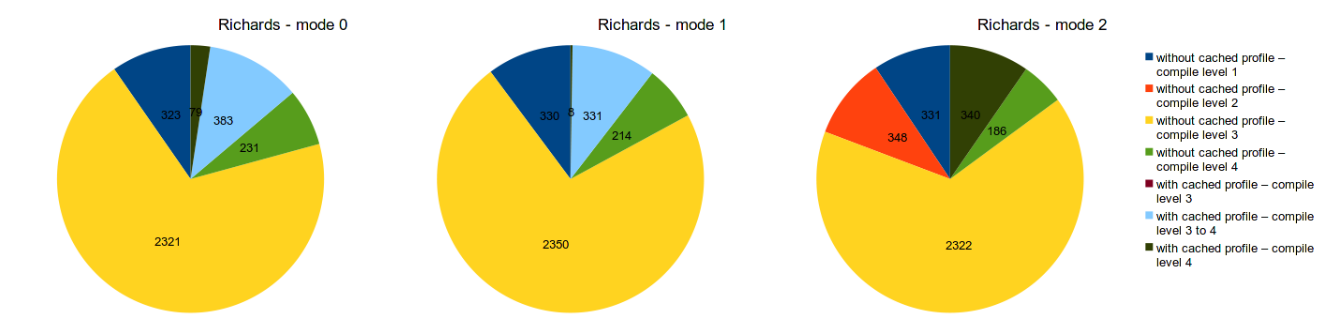
\includegraphics[width=1.0\textwidth]{figures/richards_compilations.png}
    \caption{Ratio of compilations Octane Richards benchmark}
    \label{f:richards_compilations}
  \end{center}
\end{figure}
% --------------------------- Compilation cake Richards ------------------
\begin{figure}[ht]
  \begin{center}
    \centering
    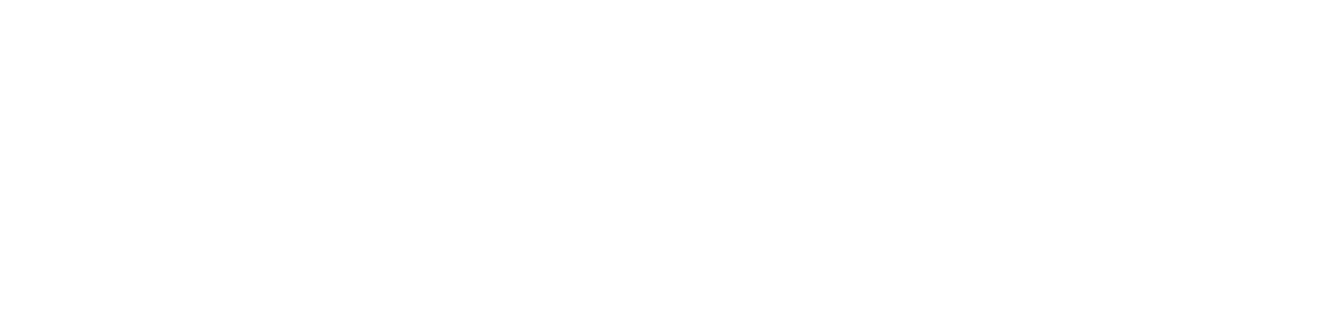
\includegraphics[width=1.0\textwidth]{figures/deltablue_compilations.png}
    \caption{Ratio of compilations Octane Deltablue benchmark}
    \label{f:deltablue_compilations}
  \end{center}
\end{figure}
% --------------------------- Compilation cake Richards ------------------
\begin{figure}[ht]
  \begin{center}
    \centering
    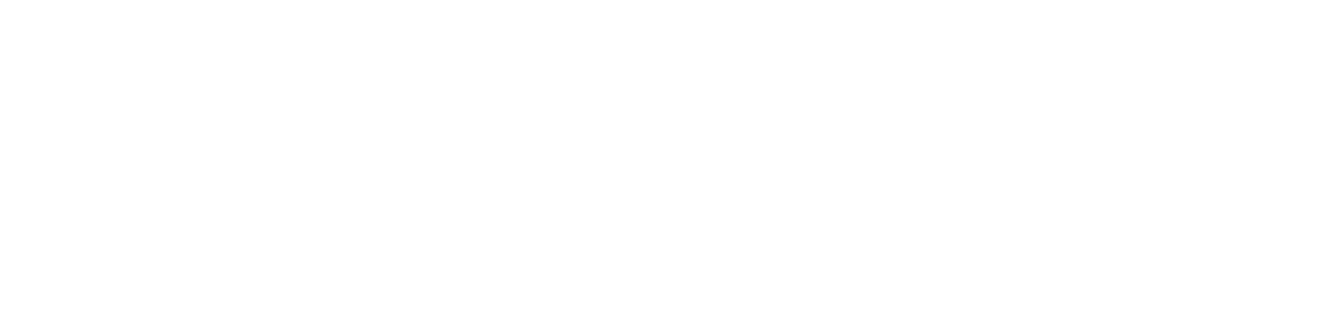
\includegraphics[width=1.0\textwidth]{figures/earleyboyer_compilations.png}
    \caption{Ratio of compilations Octane EarleyBoyer benchmark}
    \label{f:earleyboyer_compilations}
  \end{center}
\end{figure}
% --------------------------- Compilation cake Richards ------------------
\begin{figure}[ht]
  \begin{center}
    \centering
    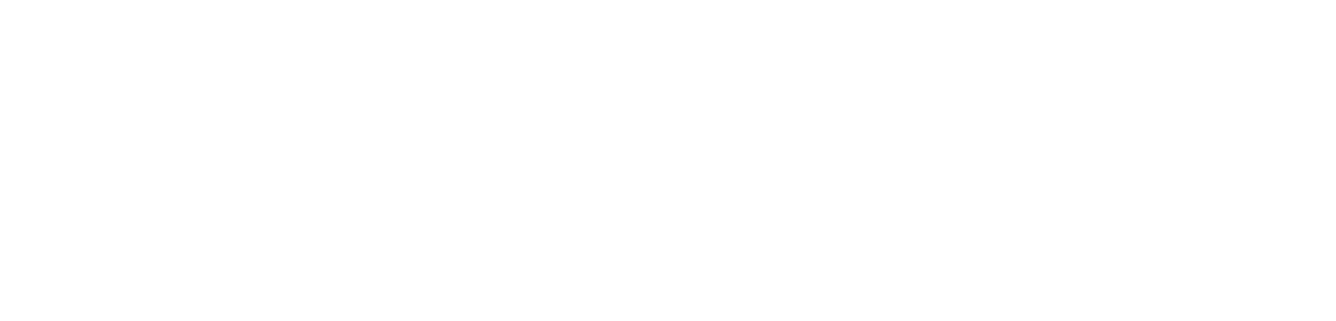
\includegraphics[width=1.0\textwidth]{figures/navierstokes_compilations.png}
    \caption{Ratio of compilations Octane NavierStokes benchmark}
    \label{f:navierstokes_compilations}
  \end{center}
\end{figure}
% --------------------------- Compilation cake compress ------------------
\begin{figure}[ht]
  \begin{center}
    \centering
    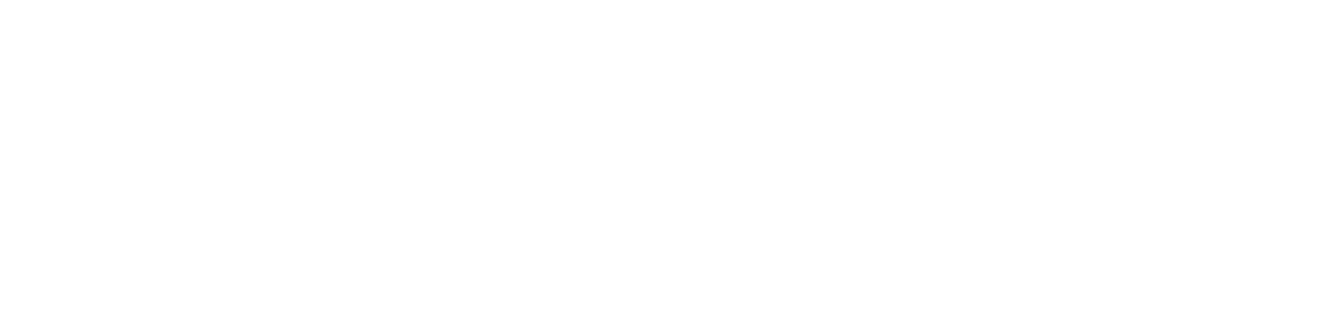
\includegraphics[width=1.0\textwidth]{figures/compress_compilations.png}
    \caption{Ratio of compilations SPECjvm compress benchmark}
    \label{f:compress_compilations}
  \end{center}
\end{figure}
% --------------------------- Compilation cake sparse.large ------------------
\begin{figure}[ht]
  \begin{center}
    \centering
    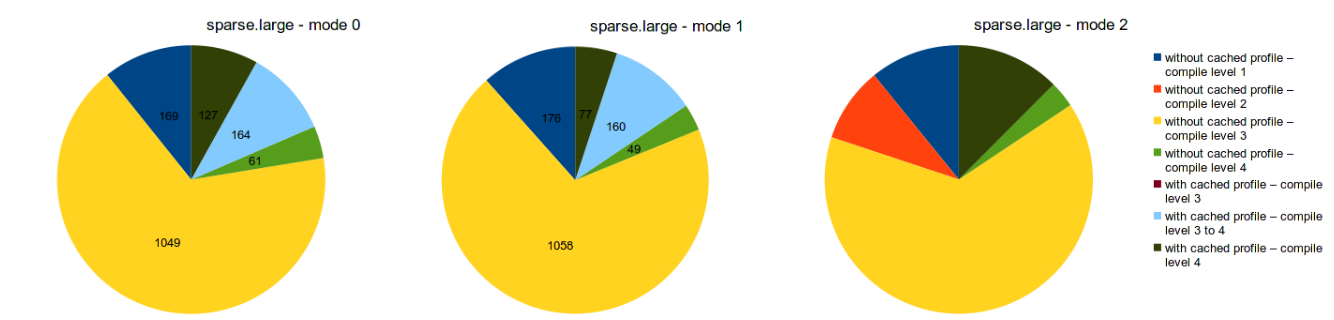
\includegraphics[width=1.0\textwidth]{figures/sparselarge_compilations.png}
    \caption{Ratio of compilations SPECjvm sparse.large benchmark}
    \label{f:sparselarge_compilations}
  \end{center}
\end{figure}
\clearpage
\section{Effect of interpreter profiles}
\label{s:perf_interpreter_profiles}
Our system makes use of two types of cached profiles. Profiles that are gathered by the interpreter and used by the C1 compiler and profiles that are gathered by a C1 compiled method and used when compiling with C2.
\\\\
We added a HotSpot flag that allows us to specify the minimum level of a compilation that dumps profiles (\texttt{-XX:DumpProfilesMinTier=}level).
Previous measurements were done using Level 3 which dumps profiles during C1 and C2 compilations.
\\\\
However, we are also interested how the system performance changes when only C2 compiler profiles are used. The system will then only use cached profiles where a C2 compilation took place in the previous profile generation run. We use the same setup as before and run the individual SPECjvm (see Figure \ref{f:others_warmup_wo_i} and Octane (see Figure \ref{f:octane_wo_i} benchmarks. 
\\\\
Most of the benchmarks do not show significantly different results compared to Section \ref{s:perf_benchmark}, where both types of cached profiles where used. There are a few benchmarks where individual modes now improve the performance while having a performance drop when using C1 and C2 profiles (e.g. NavierStokes \texttt{Mode 0}). But we also experience the other way around for example in benchmark Splay \texttt{Mode 2}. In these individual cases, we believe that for example a benchmarks C1 compilation does not profit from having cached profiles and therefore using them will even decrease performance. This happens because methods are first compiled by using cached profiles and after ten deoptimizations are compiled using generated profiles.
\\\\
The results let us conclude that the performance differences to the baseline are mostly due to the code quality of C2 compilations. Even though the number of C1 compilations is usually a lot higher than the number of C2 compilations, C2 compilations seem more crucial to the methods performance.
Since C2 is the maximum compilation level, a program might spend most of it's time in C2 compiled code.
\\\\
This again shows that it is very hard to predict JVM performance.
\begin{figure}[ht]
  \begin{center}
    \centering
    \includegraphics[width=1.0\textwidth]{figures/all_warmup_variation_wo_i.png}
    \caption{Relative performance from baseline for all SPECjvm benchmarks without using cached interpreter profiles}
    \label{f:others_warmup_wo_i}
  \end{center}
\end{figure}
\begin{figure}[ht]
  \begin{center}
    \centering
    \includegraphics[width=1.0\textwidth]{figures/octane_variation_wo_i.png}
    \caption{Relative performance from baseline for all Octane benchmarks without using cached interpreter profiles}
    \label{f:octane_wo_i}
  \end{center}
\end{figure}
\clearpage
\section{Effect of intrinsified methods}
\label{s:perf_intrinsics}
This chapter takes a quick look at the influence of method intrinsics.
The HotSpot JVM does not compile some common standard library methods. Instead it emits hand-written assembler code.
TODO
%
% \begin{figure}[ht]
%   \begin{center}
%     \centering
%     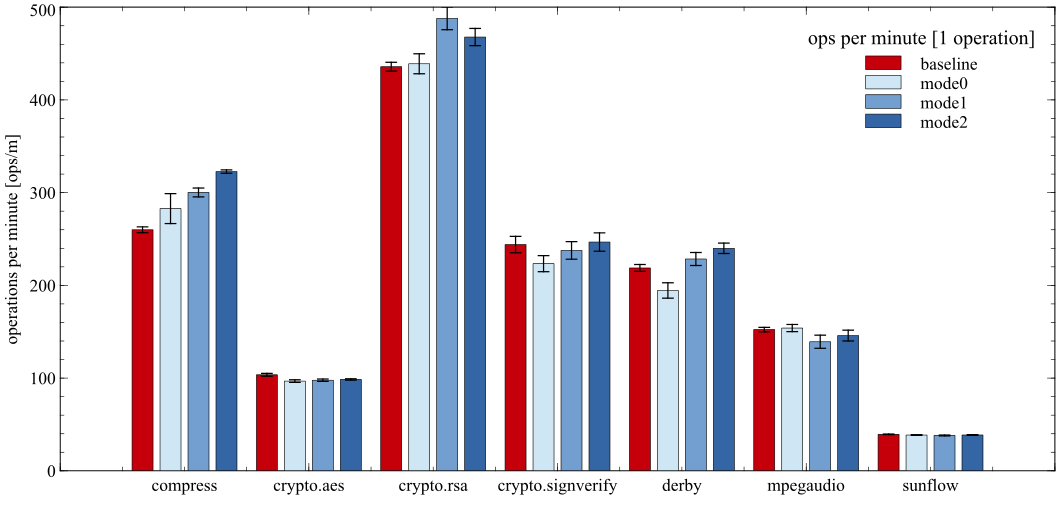
\includegraphics[width=1.0\textwidth]{figures/others_warmup_nointrinsics.png}
%     \caption{SPECjvm benchmarks on all different modes without intrinsified methods}
%     \label{f:others_warmup_nointrinsics}
%   \end{center}
% \end{figure}
%
% \begin{figure}[ht]
%   \begin{center}
%     \centering
%     \includegraphics[width=1.0\textwidth]{figures/scimark_warmup_nointrinsics.png}
%     \caption{SPECjvm scimark benchmarks on all different modes without intrinsified methods}
%     \label{f:scimark_warmup_nointrinsics}
%   \end{center}
% \end{figure}
%
%
% \begin{figure}[ht]
%   \begin{center}
%     \centering
%     \includegraphics[width=1.0\textwidth]{figures/all_warmup_nointrinsics_variation.png}
%     \caption{Relative performance from baseline for all SPECjvm benchmarks without intrinsified methods}
%     \label{f:all_warmup_nointrinsics_variation}
%   \end{center}
% \end{figure}


\chapter{Possible Improvements}
\label{c:improvements}
While this thesis provides a first look on implementing a system to reuse profiles from previous JVM runs it leaves room for several improvements.
\begin{itemize}
  \item The datastructure of the cached profiles is a simple C heap array. The lookup is $O(n)$ with $n$ being the number of cached method compilations. This could be improved to $O(nlog(n))$ by using a more complex tree-like data structure.
  \item Additionally, all method compilations get dumped and stored. The system could be improved in a way, so only the last compilation record of a method is kept in the file. This would decrease the size of the cached profile file and decrease the parsing time.
  \item Currently, only the profiles from a single run are used. A possible improvement is to use multiple executions for gathering the cached profiles and merge the profiling information to achieve even more complete profiles.
  \item We think it could also be beneficial to be able to modify the cached profile. That would allow the JVM user to manually improve profiling information by using his knowledge of the method execution which might not be available to the compiler.
\end{itemize}


\chapter{Conclusion}
\label{c:conclusion}
Modern Java Virtual Machines (JVM) like HotSpot gather profiling information about executed methods to improve the quality of the compiled code.
This thesis presents several approaches to reuse profiling information, that have been dumped to disk in previous executions of the JVM.
\\\\
The expected advantage is a faster warmup of the Virtual Machine, because the JVM does not need to spend time profiling the code and can use cached profiles directly.
Furthermore, since the cached profiles originate from previous compilations, where extensive profiling already happened, compilations using these profiles produce more optimized code, which decreases the amount of deoptimizations.
\\\\
We show, using two benchmark suites, that cached profiles can indeed improve warmup performance and significantly lower the amount of deoptimizations.
Therefore, we believe, that cached profiles are a valuable asset in scenarios where a fast JVM warmup is needed and performance fluctuations during tiered compilation want to be avoided.
\\\\
In addition, we tested individual benchmarks for the impact of cached profiles on the load of the compile queue, the amount and type of compilations, and the time spent in the compilers. The results show, that neither of them gives one-to-one correspondence between the examined factor and performance. However, the results provide indications, where the performance increase or decrease could come from.
\\\\
The functionality is implemented in the HotSpot JVM (openJDK9). It provides the user of the JVM several choices on how to use the system and allows fine-grained selection of the cached methods.

% -------------------------------------------------------------------------------------------------
% Appendices (if needed)
% -------------------------------------------------------------------------------------------------
\appendix
\chapter{Appendix}
\label{c:appendix}
\newpage
\section{Tiered Compilation Thresholds}
\label{a:compilethresholds}
\begin{table}[h]
  \centering
 % \caption{}
  \label{t:compilethresholds}
  \begin{center}
    \begin{tabular}{| l | p{9.0cm} | r | }
       \hline
       \textbf{flag} & \textbf{description} & \textbf{default} \\ \hline\hline
       CompileThresholdScaling & number of interpreted method invocations before (re-)compiling & 1.0\\ \hline
       Tier0InvokeNotifyFreqLog & Interpreter (tier 0) invocation notification frequency & 7\\ \hline
       Tier2InvokeNotifyFreqLog & C1 without MDO (tier 2) invocation notification frequency & 11 \\ \hline
       Tier3InvokeNotifyFreqLog & C1 with MDO profiling (tier 3) invocation notification frequency & 10 \\ \hline
       Tier23InlineeNotifyFreqLog & Inlinee invocation (tiers 2 and 3) notification frequency & 20 \\ \hline
       Tier0BackedgeNotifyFreqLog & Interpreter (tier 0) invocation notification frequency & 10 \\ \hline
       Tier2BackedgeNotifyFreqLog & C1 without MDO (tier 2) invocation notification frequency & 14 \\ \hline
       Tier3BackedgeNotifyFreqLog & C1 with MDO profiling (tier 3) invocation notification frequency & 13 \\ \hline
       Tier2CompileThreshold & threshold at which tier 2 compilation is invoked & 0 \\ \hline
       Tier2BackEdgeThreshold & Back edge threshold at which tier 2 compilation is invoked & 0 \\ \hline
       Tier3InvocationThreshold & Compile if number of method invocations crosses this threshold & 200 \\ \hline
       Tier3MinInvocationThreshold & Minimum invocation to compile at tier 3 & 100 \\ \hline
       Tier3CompileThreshold & Threshold at which tier 3 compilation is invoked (invocation minimum must be satisfied) & 2000 \\ \hline
       Tier3BackEdgeThreshold & Back edge threshold at which tier 3 OSR compilation is invoked & 60000 \\ \hline
       Tier4InvocationThreshold & Compile if number of method invocations crosses this threshold & 5000 \\ \hline
       Tier4MinInvocationThreshold & Minimum invocation to compile at tier 4 & 600 \\ \hline
       Tier4CompileThreshold & Threshold at which tier 4 compilation is invoked (invocation minimum must be satisfied) & 15000 \\ \hline
       Tier4BackEdgeThreshold & Back edge threshold at which tier 4 OSR compilation is invoked & 40000 \\ \hline
    \end{tabular}
  \end{center}
\end{table}


% -------------------------------------------------------------------------------------------------
% Bibliography
% -------------------------------------------------------------------------------------------------
\addcontentsline{toc}{chapter}{Bibliography}
\bibliography{bibliography}

\end{document}
